%%%%%%%%%%%%%%%%%%%%%%%%%%%%%%%%%%%%%%%%%%%%%%%%%%%%%%%%%%%%%%%%%%%%%%%%%%%%%%%%
%2345678901234567890123456789012345678901234567890123456789012345678901234567890
%        1         2         3         4         5         6         7         8

\documentclass[conference]{IEEEtran} % [letterpaper, 10 pt, conference]{ieeeconf}  % Comment this line out if you need a4paper

%\documentclass[a4paper, 10pt, conference]{ieeeconf}      % Use this line for a4 paper

\IEEEoverridecommandlockouts                              % This command is only needed if 
                                                          % you want to use the \thanks command

\overrideIEEEmargins                                      % Needed to meet printer requirements.

%In case you encounter the following error:
%Error 1010 The PDF file may be corrupt (unable to open PDF file) OR
%Error 1000 An error occurred while parsing a contents stream. Unable to analyze the PDF file.
%This is a known problem with pdfLaTeX conversion filter. The file cannot be opened with acrobat reader
%Please use one of the alternatives below to circumvent this error by uncommenting one or the other
%\pdfobjcompresslevel=0
%\pdfminorversion=4

% See the \addtolength command later in the file to balance the column lengths
% on the last page of the document

% ==================================================================================
\usepackage{graphics} % for pdf, bitmapped graphics files
\usepackage{epsfig} % for postscript graphics files
%\usepackage{mathptmx} % assumes new font selection scheme installed
%\usepackage{times} % assumes new font selection scheme installed
\usepackage{amsmath} % assumes amsmath package installed
\usepackage{amssymb}  % assumes amsmath package installed
\usepackage{amsfonts} % assumes amsfonts package installed
\usepackage{epstopdf}
\usepackage{color}
\usepackage{comment}
\usepackage{algorithm}
\usepackage{algorithmic}
%\usepackage{algpseudocode}
\renewcommand{\algorithmicrequire}{\textbf{Input:}}  % Use Input in the format of Algorithm  
\renewcommand{\algorithmicensure}{\textbf{Output:}} % Use Output in the format of Algorithm  
%===================================================================================

\newtheorem{example}{Example}
\newtheorem{remark}{Remark}
\newtheorem{definition}{Definition}
\newtheorem{theorem}{Theorem}
\newtheorem{lemma}{Lemma}
\newtheorem{proposition}{\bf Proposition}


%============================================================================
\def \BN {{\em BN}}
\def \BNs {{\em BNs}}
\def \BCN {{\em BCN}}
\def \BCNs {{\em BCNs}}
\def \Pe {{\tt Pe}}
\def \Pv {{\tt Pv}}
\def \Spe {{\tt Spe}}
\def \Ce {{\tt Ce}}
\def \Cv {{\tt Cv}}
\def \Lce {{\tt Lce}}
\def \Ded {{\tt Ded}}
\newcommand{\rev}[1]{{\color{red}{#1}}}


%=======================================================================
\newcommand{\tl}[1]{\textcolor{blue} {TL: #1 :TL} }

%========================================================================

\title{\LARGE \bf
Online Observability of Boolean Control Networks*
}

\begin{comment}


\author{Guisen Wu$^{1}$ and Liyun Dai$^{1}$ and Taolue Chen$^{2}$% <-this % stops a space
\thanks{*This work was not supported by any organization}% <-this % stops a space
\thanks{$^{1}$Albert Author is with Faculty of Electrical Engineering, Mathematics and Computer Science,
        University of Twente, 7500 AE Enschede, The Netherlands
        {\tt\small albert.author@papercept.net}}%
\thanks{$^{2}$Bernard D. Researcheris with the Department of Electrical Engineering, Wright State University,
        Dayton, OH 45435, USA
        {\tt\small b.d.researcher@ieee.org}}%
}
\end{comment}

\author{\IEEEauthorblockN{Guisen Wu\quad  Liyun Dai*\thanks{*Corresponding author} \quad Zhiming Liu}
\IEEEauthorblockA{\textit{RISE \& School of Computer and Information Science,}\\ \textit{Southwest University}\\
Chongqing, China \\
$\{$wgs233,dailiyun,zhimingliu88$\}$@swu.edu.cn}
\and
\IEEEauthorblockN{Taolue Chen}
\IEEEauthorblockA{\textit{Department of Computer Science and Information Systems} \\
	\textit{Birkbeck, University of London}\\
taolue@dcs.bbk.ac.uk}
\and
\IEEEauthorblockN{Jun Pang}
\IEEEauthorblockA{\textit{Faculty of Science, Technology and Communication} \\
	\textit{University of Luxembourg}\\
jun.pang@uni.lu}
\and
\IEEEauthorblockN{Hongyang Qu}
\IEEEauthorblockA{\textit{Department of Automatic Control and Systems Engineering} \\
	\textit{University of Sheffield}\\
h.qu@sheffield.ac.uk}
}

%\end{comment}

\begin{document}



\maketitle
\thispagestyle{empty}
\pagestyle{empty}


%%%%%%%%%%%%%%%%%%%%%%%%%%%%%%%%%%%%%%%%%%%%%%%%%%%%%%%%%%%%%%%%%%%%%%%%%%%%%%%%
\begin{abstract}

Four types of observability of Boolean control networks (\BCNs) have been proposed to solve different problems. However, all of them are offline observabilities that we can not adjust the input sequence by observing the output sequence in the process of determining the initial state of \BCNs. In this paper, we firstly propose the online observability that it can determine the initial state of \BCNs\ dynamically without presupposing its initial state. The online observability accomplishes this task by deciding input sequence and observing out sequence in every time step. The node values of \BCNs\ update at discrete time, then we use the time step to represent the discrete time. Compared with offline observabilities, the online obsevability can determine the initial state of some biological systems which can be checked at most once. %We define the concepts of deduce function, $K$ steps deterministic and the formal definition of online observability of BCNs. We also define the supertree and directed graph to determine online observability for BCNs. 
\end{abstract}


\begin{keywords}

Boolean control networks, online observability, directed graph, supertree%, find shortest path, avoid entering critical states. 

\end{keywords}

%\section{ssssss}
\label{sec;one}
ssssssss

ss

s

s
s

d
d
f

% !Mode\dots ``TeX:UTF-8''
% !TEX root = ../bare_jrnl.tex


\section{Introduction}
\label{sec:intro}


\IEEEPARstart{I}n 1960s, Nobel Prize laureates Jacob and Monod~\cite{Jacob1961Genetic} found that ``Any cell contains a number of regulatory genes that act as switches and can turn one another on and off. If genes can turn one another on and off, then you can have genetic circuits.'' Inspired by these Boolean-type actions in genetic circuits, Boolean networks (\BNs) were firstly proposed by Kauffman \cite{Kauffman1968Metabolic} for modeling nonlinear and complex biological systems. 

{\BNs} are a type of discrete-time dynamical systems which can be represented as directed graphs. In a BN, each node has only two values ``0" and ``1", and they can change in different time points.  For a node $n_i$, we use $n_i(t)$ to denote its value at time $t$.
In general, $n_i(t+1)$ is determined by a logical function of $n_j(t),\ldots,n_p(t)$ if  there are  edges from $n_j,\ldots,n_p$ to $n_i$.  
%The logical operators used in  the logical functions include AND, OR, NO, XOR.  
Some general descriptions of the \BNs\ and their applications to biological systems can be found in~\cite{Kauffman1968Metabolic}. There exists a large number of  systems, both natural and artificial, which are modelled as \BNs, e.g. ~\cite{Akutsu2000Inferring, Shmulevich2002From, Faur2006Dynamical,Green2007The,Lou2010Multi}.
 \JP{Here, what do you mean by `systems works'?}

\BNs\ can be naturally extended to Boolean control networks (\BCNs) with external regulations and perturbations~\cite{Ideker2001A}. \BCNs\ have been applied to  various real-life problems. Cases of application can be found in 
structural and functional analysis of signaling and regulatory networks~\cite{Kaufman1999A, Klamt2006A}, 
abduction based drug target discovery~\cite{Biane2017Abduction}, 
and pursuing evasion problems in polygonal environments~\cite{Thunberg2011A}.
%
There are three kinds of nodes in \BCNs:  {\em input-nodes}, {\em state-nodes}  and {\em output-nodes}. At any moment of time each node takes a Boolean value.  The value of an output-node at time point $t$ (where $t\geq 0$)  depends on the values of state-nodes at time $t$, but the value of a  state-node at time point $t+1$  is determined by a  Boolean function of the values of the input-nodes and state-nodes at time point $t$. However,  we can only control the  values of the input-nodes and observe those of the output-nodes. Thus,  we cannot observe how   the values of the state-nodes change from time to time. Therefore, it is important to find a way to determine the initial values of the state-nodes at $0$ after observing a sequence of values of  input-nodes and their corresponding  values of the output-nodes. This is in general known as the {\em observability} of a \BCN.



Observability is one of the two basic  properties related to  the control-theoretic problems of \BCNs. The other is known as {\em controllability}. The work in ~\cite{Akutsu2007Control} shows that the problem of determining the controllability of \BCNs\ is {NP}-hard. Moreover, it  points out that ``One of the major goals of systems biology is to develop a control theory for complex biological systems.''  Since then, research on  controllability and observability of \BNs\ and \BCNs\ has drawn a great attention, e.g. \cite{cheng2009controllability, Zhao2010Input, Cheng2011Identification, Cheng2011Analysis} and \cite{Fornasini2013Observability}. %There, it is further noted that the controllability and observability are the basic control-theoretic problems of \BCNs. % Among these studies, \emph{semi-tensor product} (\STP) is one of useful tools to deal with  

 The concept of observability was first proposed in~\cite{cheng2009controllability}. It is mainly about how  to determine  the values of the  state-nodes  of a \BCN\  at time $0$ from the values of  input-nodes  and output-nodes at a sequence of time points $0,\ldots, k$. After that, four types of observability have been investigated in the literature,
 together with their corresponding determining algorithms, which we will discuss below.

\begin{figure}[!t]
      \centering
      \framebox{\parbox{3in}{
		\centerline{\includegraphics[scale=0.17]{figures/Fig10.png}}
	}}
      
      \caption{The relationship of inputs, states and outputs.}
      \label{fig:10}
  \end{figure}

Given a \BCN\ with $\ell$ input-nodes $(\mathsf{i}_1,\ldots, \mathsf{i}_\ell)$, $m$ state-nodes $(\mathsf{s}_1,\ldots, \mathsf{s}_m)$ and $n$ output notes  $(\mathsf{o}_1,\ldots, \mathsf{o}_n)$,  we use an {\em input vector} $\mathsf{i}(t)=(\mathsf{i}_1(t)\ldots\mathsf{i}_\ell (t))$, a {\em state vector} $\mathsf{s}(t)=(\mathsf{s}_1(t), \ldots \mathsf{s}_m(t))$ and an {\em output  vector} $\mathsf{o}(t)=(\mathsf{o}_1(t) \ldots \mathsf{o}_n(t))$  to represent an assignment of Boolean values to the  input-nodes, state-nodes and  output-nodes at $t$, respectively.  We call them an {\em input}, a {\em state} and an {\em output} of the \BCN\ at time time $t$. As  illusreated by Fig.~\ref{fig:10},  the state $\mathsf{s}(t+1)$ at time $t+1$ is determined by the input   $\mathsf{i}(t)$ and state $\mathsf{s}(t)$ at $t$  and the output   $\mathsf{o}(t)$ by the state  $\mathsf{s}(t)$.  We call a state $\mathsf{s}(0)$ at time $0$ an {\em initial state}. Thus, for any $k>0$ and any  initial state $\mathsf{s}(0)$, the states  $\mathsf{s}(1),\ldots, \mathsf{s}(k)$ and the output sequence $\mathsf{o}(1)\ldots, \mathsf{o}(k)$ are  determined by an  input sequence $\mathsf{i}(0),\ldots, \mathsf{i}(k-1)$.
%That is for a given  \BCN\  $\BB$,  $\mathsf{o}(0)\mathsf{o}(1)\ldots\mathsf{o}(k)$ is decide by $\mathsf{s}(0)$ and the sequence $\mathsf{i}(0)\mathsf{i}(1)\ldots\mathsf{i}(k-1)$. 
%
The four existing notions of observability of \BCNs\ can thus be described as follows. 
\begin{enumerate}
\item The  {\bf type-I}  observability was proposed in 2009 \cite{cheng2009controllability}. It states that a \BCN\ $\BB$ is observable if for any initial state   $\mathsf{s}(0)$ there exists an input sequence  $\mathsf{i}(0),\mathsf{i}(1),\ldots,\mathsf{i}(k-1)$ which can  distinguish $\mathsf{s}(0)$ from any other initial state $s'(0)$. That is,  given an initial state $\mathsf{s}(0)$, there is an input sequence $\mathsf{I}(k)=\mathsf{i}(0),\mathsf{i}(1),\ldots,\mathsf{i}(k-1)$ such that  for any  $\mathsf{s}'(0)$ which is different from $\mathsf{s}(0)$, the output sequence  $\mathsf{O}(k)=\mathsf{o}(0),\mathsf{o}(1),\ldots,\mathsf{o}(k)$ produced by  $\mathsf{s}(0)$ and $I(k)$ is different the output sequence  $\mathsf{O}'(k)=\mathsf{o}'(0),\mathsf{o}'(1),\ldots, \mathsf{o}'(k)$ produced by  $\mathsf{s}'(0)$ and $\mathsf{I}(k)$.

\item The  {\bf type-II} observability was proposed in 2010 \cite{Zhao2010Input}. It states that a \BCN\ $\BB$ is observable if for every two different initial states $\mathsf{s}(0)$ and $\mathsf{s}'(0)$, there exists an input \JP{`inout'? or `input'?} sequence $\mathsf{i}(0),\mathsf{i}(1),\ldots, \mathsf{i}(k-1)$ that can distinguish $\mathsf{s}(0)$ and $\mathsf{s}'(0)$. More precisely speaking,  for any pair of different initial  $\mathsf{s}(0)$ and $\mathsf{s}'(0)$, \JP{Why use $\mathsf{s}^{y}(0)$?}
there exists an input sequence  $\mathsf{i}(0),\mathsf{i}(1),\ldots,\mathsf{i}(k-1)$ such that the output sequences $\mathsf{o}(0),\mathsf{o}(1),\ldots,\mathsf{o}(k)$ and  $\mathsf{o}'(0),\mathsf{o}'(1),\ldots,\mathsf{o}'(k)$ corresponding to  the different initial states  $\mathsf{s}(0)$ and $\mathsf{s}'(0)$, respectively, are different.
	
\item The  {\bf type-III} observability was proposed in 2011 \cite{Cheng2011Identification}.  It states that a \BCN\ $\BB$ is observable if for any $k>0$ there is a sequence $\mathsf{i}(0),\mathsf{i}(1),\ldots, \mathsf{i}(k-1)$ that distinguishes every pair of different initial states. This means that in $\BB$, there exists an input \JP{`inout'?} sequence  $\mathsf{i}(0),\mathsf{i}(1), \ldots,\mathsf{i}(k-1)$ such that for any two different initial states $\mathsf{s}(0)$ and $\mathsf{s}'(0)$, the output sequence $\mathsf{o}(0),\mathsf{o}(1), \ldots, \mathsf{o}(k)$  corresponding to  $\mathsf{s}(0)$  is different from the output sequence  $\mathsf{o}'(0),\mathsf{o}'(1),\ldots, \mathsf{o}'(k)$ corresponding to $\mathsf{s}'(0)$.
\JP{Please don't change notations. Stick to $s(0)$ and $s'(0)$. $\mathsf{s}^{x}(0)$ and $\mathsf{s}^{y}(0)$ are somehow strange.}
	
\item  The  {\bf type-IV}  observability was  proposed in 2013 \cite{Fornasini2013Observability}. It states that a \BCN\ $\BB$ is observable if every sufficient long $\mathsf{i}(0)$$\mathsf{i}(1)\ldots$$\mathsf{i}(k-1)$ genertaes different output sequences  from different initial states. Precisely speaking, there is a big enough number $M$, for every  input sequence $\mathsf{i}(0),\mathsf{i}(1),\ldots, \mathsf{i}(k-1)$ which is not shorter than $M$, the output sequences $\mathsf{o}(0), \mathsf{o}(1), \ldots, \mathsf{o}(k)$ and  $\mathsf{o}'(0), \mathsf{o}'(1), \ldots, \mathsf{o}'(k)$ produced by the inout sequence from every two different initial states $\mathsf{s}(0)$ and $\mathsf{s}'(0)$, respectively, are different.
\end{enumerate}
 We will give the formal definitions of these four types of observability and discussion their relations in Section~\ref{sec:pre}.
 \JP{So far, I don't see a clear difference among the first three types from the above description.}

%\JP{Here, you need an introductory sentence on why algorithms are needed.}
%Four types of observability develop different algorithms to determine $\mathsf{s}(0)$ of \BCN. 
Let $\mathsf{S}(t)$ denote the set of possible valuations of $\mathsf{s}(t)$.

For the {\bf type-I} observability, if a \BCN\ is observable then we can determine its $\mathsf{s}(0)$ by following procedure. 
\begin{description}
	\item[Step 1] We infer $\mathsf{S}(0)$ by the $\mathsf{o}(0)$ based on the relation of $\mathsf{o}(t)$ and $\mathsf{s}(t)$. For every $\mathsf{s}^x (0)\in\mathsf{S}(0)$, there exists an input sequence $\mathsf{i^x }(0),\mathsf{i}^x (1),\ldots,\mathsf{i}^x (k-1)$ which can distinguish $\mathsf{s}^x (0)$ from any other initial state.
	\item[Step 2] We choose a $\mathsf{s}^x (0)$ from $\mathsf{S}(0)$, and input its corresponding $\mathsf{i}^x (0),\mathsf{i}^x (1),\ldots,\mathsf{i}^x (k-1)$. If the initial state of \BCN\ $\mathsf{s}(0)=\mathsf{s}^x (0)$, we can determine $\mathsf{s}(0)$ from the output sequence of \BCN, else we reset the state of the \BCN\ by $\mathsf{s}(0)$ and repeat this procedure.
	
\end{description}

 For the {\bf type-II} observability, if a \BCN\ is observable then we can determine its $\mathsf{s}(0)$ by following procedure. 
\begin{description}
	\item[Step 1] We infer $\mathsf{S}(0)$ by the $\mathsf{o}(0)$ based on the relation of $\mathsf{o}(t)$ and $\mathsf{s}(0)$. 
	\item[Step 2] We input a $\mathsf{i}(0),\mathsf{i}(1),\ldots,\mathsf{i}(k-1)$ which can help us further determine $\mathsf{S}(0)$ by observing the output sequence of \BCN. If $|\mathsf{S}(0)|$ becomes $1$, we can determine $\mathsf{s}(0)$, else reset the state of the \BCN\ by $\mathsf{s}(0)$ and repeat this procedure.
\end{description}

 For the {\bf type-III} observability, if a \BCN\ is observable then we can determine its $\mathsf{s}(0)$ by inputing the $\mathsf{i}(0),\mathsf{i}(1),\ldots,\mathsf{i}(k-1)$ that distinguish every pair of different initial states and observing the output sequence of \BCN.

For the {\bf type-IV} observability, if a \BCN\ is observable then we can determine its $\mathsf{s}(0)$ by inputing any sufficient long $\mathsf{i}(0),\mathsf{i}(1),\ldots,\mathsf{i}(k-1)$ and observing the output sequence of \BCN.
%{\color{red} (13)}

Loosely speaking, different ways to determine $\mathsf{s}(0)$ are proposed for different applications, and the four types of observability present whether a \BCN\ can be determined by these four ways respectively. When the $\mathsf{s}(0)$ of \BCN\ can be reset, we use the way corresponding to {\bf type-I} or {\bf type-II} to determine $\mathsf{s}(0)$. The {\bf type-IV} observability is proposed to research the reconstructibility of \BCN. The {\bf type-III} observability is proposed to research the identification of \BCN. And in the identification problem of \BCNs, a \BCN\ is identifiable iff it is controllable and its $\mathsf{s}(0)$ can be determined when $\mathsf{s}(0)$ can not be reset.%And the second observability is the necessary and sufficient condition of determining $\mathsf{s}(0)$ by taking the determining procedure once. 
\JP{What applications?}

In this paper, we propose a new way to determine $\mathsf{s}(0)$ when it can not be reset. It is better than the way corresponding to {\bf type-III} observability%address the necessary and sufficient condition of determining $\mathsf{s}(0)$ by taking the determining process once to make \BCN\ be able to apply to more applications.
%\JP{Here, `necessary and sufficient condition' appears for the first time. What are their precise definitions?}
%Naturally there is a procedure to determine $\mathsf{s}(0)$  which is described as follows.
%\JP{Why in this way it can be applied to more applications?}
%It enriches the control-theory of \BCNs, it can help us determine the $\mathsf{s}(0)$ of some \BCNs\ which can not be determined before.

%\begin{problem}
%\label{pro:1}
%For a given \BCN\ $\BB$, whether its initial state $\mathsf{s}(0)$ can be determined by carrying on determining procedure once?
%\end{problem}

%Although, these four existing notions of observability can help us study some information about $\mathsf{s}(0)$ we need. 
%The problem means that whether the $\mathsf{s}(0)$ can be determined if the determining procedure can do at most once. %only third and fourth ones  can  determine the $\mathsf{s}(0)$ of \BCNs.
%Only third and fourth notions of observability can help us solve the {\em Problem~\ref{pro:1}}.
% What is more, in the third observability, a \BCN\ is observable iff there is an input sequence that determines its initial state $\mathsf{s}(0)$. Thus its condition is very strong, and the condition of fourth observability is even stronger.
%However, 
%Let $\mathsf{S}(t)$ denote the set of possible valuations of $\mathsf{s}(t)$. Then naturally there is a procedure which is described as follows.
%We find that to determine $\mathsf{s}(0)$ by taking the determining procedure once we only need to complete the following procedure. 

%Informly, the procedure of our  online observability as follows. 
 %Then $\mathsf{S}(t)$ can be derived by the output sequence $\mathsf{o}(0)\mathsf{o}(1)\ldots\mathsf{o}(t)$, input sequence $\mathsf{i}(0)\mathsf{i}(1)\ldots\mathsf{i}(t-1)$ and updating rules of $\BB$.
 
 %\tl{can you make this a proper algorithm?}\gs{I have corrected this one.}
\begin{description}
	\item[Step 1] We infer $\mathsf{S}(t)$ by the $\mathsf{o}(t)$ based on the relation of $\mathsf{o}(t)$ and $\mathsf{s}(t)$.
	\item[Step 2] According to the relation of $\mathsf{i}(t)$, $\mathsf{s}(t)$ and $\mathsf{s}(t+1)$ we choose an $\mathsf{i}(t)$ which would not make every two distinct $\mathsf{s}(t)$ , $\mathsf{s}'(t)$$\in$ $\mathsf{S}(t)$ become the same state after affected by $\mathsf{i}(t)$ i.e. $\mathsf{s}(t+1)\ne\mathsf{s}'(t+1)$. Such that, for every $\mathsf{s}(t+1)\in $ $\mathsf{S}(t+1)$ there is exact one corresponding $\mathsf{s}(t)\in $ $\mathsf{S}(t)$.
	\item[Step 3] Repeating Step 1 and Step 2 until $|\mathsf{S}(t)|=1$ such that we can determine $\mathsf{s}(t)$, and for every $t>0$, for every $\mathsf{s}(t)\in \mathsf{S}(t)$ there is exact one corresponding $\mathsf{s}(t-1)\in \mathsf{S}(t-1)$, so we can determine $\mathsf{s}(t-1)$, \ldots, $\mathsf{s}(0)$.
\end{description}

%In the third observability, we can finish this procedure, thus we can determine the initial state \State$(0)$ for a \BCN. What is more, 


%Such that, the requirement for a \BCN\ to determine \State$(0)$ would be easist to satisfy. 
%{\color{red} (13)} 
 By this way, we can make full use of the output of \BCN\ to determine $\mathsf{s}(0)$, such that we can determine the \State$(0)$ which can not be determined by the way corresponding to {\bf type-III} observability. This proposition will be proved in Section~\ref{sec:online}. Then we can find more identifiable \BCNs\ and then further research the identification problem of \BCN. 
 
 We propose a new notion of observability named online observability which states that a \BCN\ is observable if the previously mentioned procedure would terminates for every \State$(0)$. Its formal definitions will be presented in Section~\ref{sec:online}. 

We call this observability online observability, because we observe $\mathsf{o}(t)$ of \BCN\ and choose $\mathsf{i}(t)$ based on the information we have collected so far at every time $t$. In contrast, in the {\bf type-III} observability we determine $\mathsf{s}(0)$ of \BCN\ by its recorded $\mathsf{o}(0)\mathsf{o}(1)\ldots\mathsf{o}(k)$ after we input $\mathsf{i}(0)\mathsf{i}(1)\ldots\mathsf{i}(k-1)$, and  we do not interfere with \BCN\ except for the logging of its inputs and outputs, thus we call it offline observability \cite{Cassar2017A}.
\JP{It is very unclear why we need this new notion and why it is supposed to be better.}
\JP{In general, the introduction lacks of a good motivation for the current research.
Can you somehow re-structure the introduction?
1. What is the context of this paper?
2. What exactly is the research problem and why it is important?
3. What are the existing solutions and why they are not sufficient?
4. What is your new solution and its main idea?
5. Why is your new solution better?
6. Any evidence to support your claim?}

 %{\color{red} (13)}

%Then, in this paper we make the following contributions. 
\medskip\noindent
{\bf Contributions.}
Firstly, we propose and formally define the online observability to help us further the identification problem of \BCN. % to address the necessary and sufficient condition of determining $\mathsf{s}(0)$ by taking the determining procedure once. %It enriches the control-theory of \BCNs. 
Secondly, we also provide a determination algorithm for the online observability. %Finally, we present some optimization brought by the online observability. Including the means to find shortest path and the approach to avoid entering critical states in the process of determining the initial states of \BCNs.  These optimization further explain the advantages of online observability of \BCNs. 

\medskip\noindent
{\bf Plan of the paper.}
The remainder of this paper is organized as follows.
 {\em Section \ref{sec:pre}} introduces necessary preliminaries about \BCNs, including the definition of \BCNs\ and four existing observability. {\em Section \ref{sec:online}} presents the definition of online observability of \BCNs. {\em Section \ref{sec:deter}} presents the determination algorithm for online observability. 
% {\em Section \ref{sec:app}} talks about some optimization brought by the online observability of \BCNs. 
 {\em Section \ref{sec:con}} ends up with the introduction of our future work.

%==============================================================================================================
% !Mode\dots ``TeX:UTF-8''
% !TEX root = ../bare_jrnl.tex

\section{Preliminaries} 
\label{sec:pre}
We now introduce the formal definition of {\BCNs} and its control theoretical properties. Throughout the paper, we use $\mathbb{B}$ to denote the set of Boolean values $\{0,1\}$ and $\mathbb{T}$ to denote the set of discrete time domain represented by the set of  natural numbers.

\subsection{Boolean Control Networks}

We take the definition in ~\cite{Ideker2001A} in which a Boolean control network (\BCN)  is given a directed graph together with two  Boolean valued functions which define the updating rules for the  values of the nodes. 

\begin{definition}[Boolean Control Network] 
\label{def:BCN}
A \BCN\ is a tuple $\BB = (I,S,O, E, \sigma, \rho, \theta)$, where 
\begin{itemize}
\item $I$, $S$ and $O$ are three finite nonempty disjoint sets of nodes (or vertices)
\begin{itemize}
	\item {\bf input nodes} $I=\{\mathsf{i}_1$,\ldots ,$\mathsf{i}_{\ell}\}$
	\item {\bf state nodes}  $S= \{\mathsf{s}_1$,\ldots ,$\mathsf{s}_m\}$, and 
	\item {\bf output nodes}: $O= \{\mathsf{o}_1$,\ldots ,$\mathsf{o}_n\}$.
	\end{itemize}	
	Each node is a Boolean variable which can take values in $\mathbb{B}$.
\item  $E \subseteq ((I\cup S)\times S)\cup (S\times O)$ is a set of edges among the nodes, and we say node $v$ directly affects node  $v'$  when $(v,v')$ is an edge in $E$.
\item The Boolean valued functions $\sigma: \mathbb{B}^\ell\times  \mathbb{B}^m \mapsto \mathbb{B}^m$ and $\rho: \mathbb{B}^m\mapsto \mathbb{B}^n$ are functions from the pairs of $\ell$-dimension and $m$-dimension vectors  of Boolean values to  the $m$-dimension vectors Boolean values and from the  $m$-dimension vectors to the  $n$-dimension vectors  of Boolean values, respectively. 
\item $\theta$ is a Boolean expression of the state nodes.
\item {\em Updating rules }:  We use 
 $\mathsf{i}= (\mathsf{i}_1,\ldots, \mathsf{i}_\ell)$, $\mathsf{s}= (\mathsf{s}_1,\ldots, \mathsf{s}_m)$ and $\mathsf{o}= (\mathsf{o}_1,\ldots, \mathsf{o}_n)$ to denote the three variables Boolean vectors corresponding  to the input nodes, state nodes and output nodes. At any time $t\in \mathbb{T}$ during the execution 
 of $\BB$, each of the variables  $\mathsf{i}$, $\mathsf{s}$ and $\mathsf{o}$  (thus each every node of $\BB$ too) take a vector of Boolean values $\mathsf{i}(t)$, $\mathsf{s}(t)$, $\mathsf{o}(t)$  in  $\mathbb{B}^\ell$, $\mathbb{B}^m$ and $\mathbb{B}^n$, respectively, such that the following equations are satisfied
\begin{equation}
\begin{split}
\mathsf{s}(t+1)=&\sigma(\mathsf{i}(t),\mathsf{s}(t))\\
\mathsf{o}(t)=&\rho(\mathsf{s}(t))
\end{split}
\label{equ:1}
\end{equation}
The above equations are also assumed to satisfy the following three conditions
\begin{enumerate}
\item $\mathsf{s}(0)$ satisfies the initial condition $\theta$;
\item the value of $\mathsf{s}_k(t+1)$ in $\mathsf{s}(t+1)$ is affected by the value  $\mathsf{i}_j(t)$ of an input node $\mathsf{i}_j \in I$ (or by the value $\mathsf{s}_j(t)$ of a state node $\mathsf{s}_j\in S$) at time $t$ only when $(\mathsf{i}_j, \mathsf{s}_k)\in E$ (or $(\mathsf{s}_j, \mathsf{s}_k)\in E$, respectively); and
\item the value $\mathsf{o}_k(t)$ in $\mathsf{o}(t)$ of an output node $\mathsf{o}_k\in O$ is affected by the value $\mathsf{s}_j(t)$ of a state node $\mathsf{s}_j\in S$ only wen $(\mathsf{s}_j,\mathsf{o}_k)\in E$.
\end{enumerate}
\end{itemize}

\end{definition}
 The two updating functions are also called the  {\bf updating rules}  of $\BB$. They define the value of the state nodes at any time by the values of the inout nodes and state nodes at the previous time point, and the the values of the output nodes by the value of the state nodes, respectively. We use $\mathcal{I}_\BB$, $\mathcal{S}_\BB$ and $\mathcal{O}_\BB$ tp denote  the sets of all possible inputs, states and outputs of $\BB$, respectively. And we will omit the subscript $\BB$ when there is no confusion. Obviously, $\mathcal{I}_\BB$, and $\mathcal{S}_\BB$ and $\mathcal{O}_\BB$ are finite with $2^\ell$, $2^m$ and $2^n$ elements, respectively. 


\begin{figure}[!t]
      \centering
      \framebox{\parbox{3in}{
		\centerline{\includegraphics[scale=0.17]{figures/Fig10.png}}
	}}
      
      \caption{The relationship of inputs, states and outputs.}
      \label{fig:10}
  \end{figure}
%===========================================================
\begin{example}\label{exa:2}
	 \begin{figure}[thpb]
		\centering
		\framebox{\parbox{3in}{
				\centerline{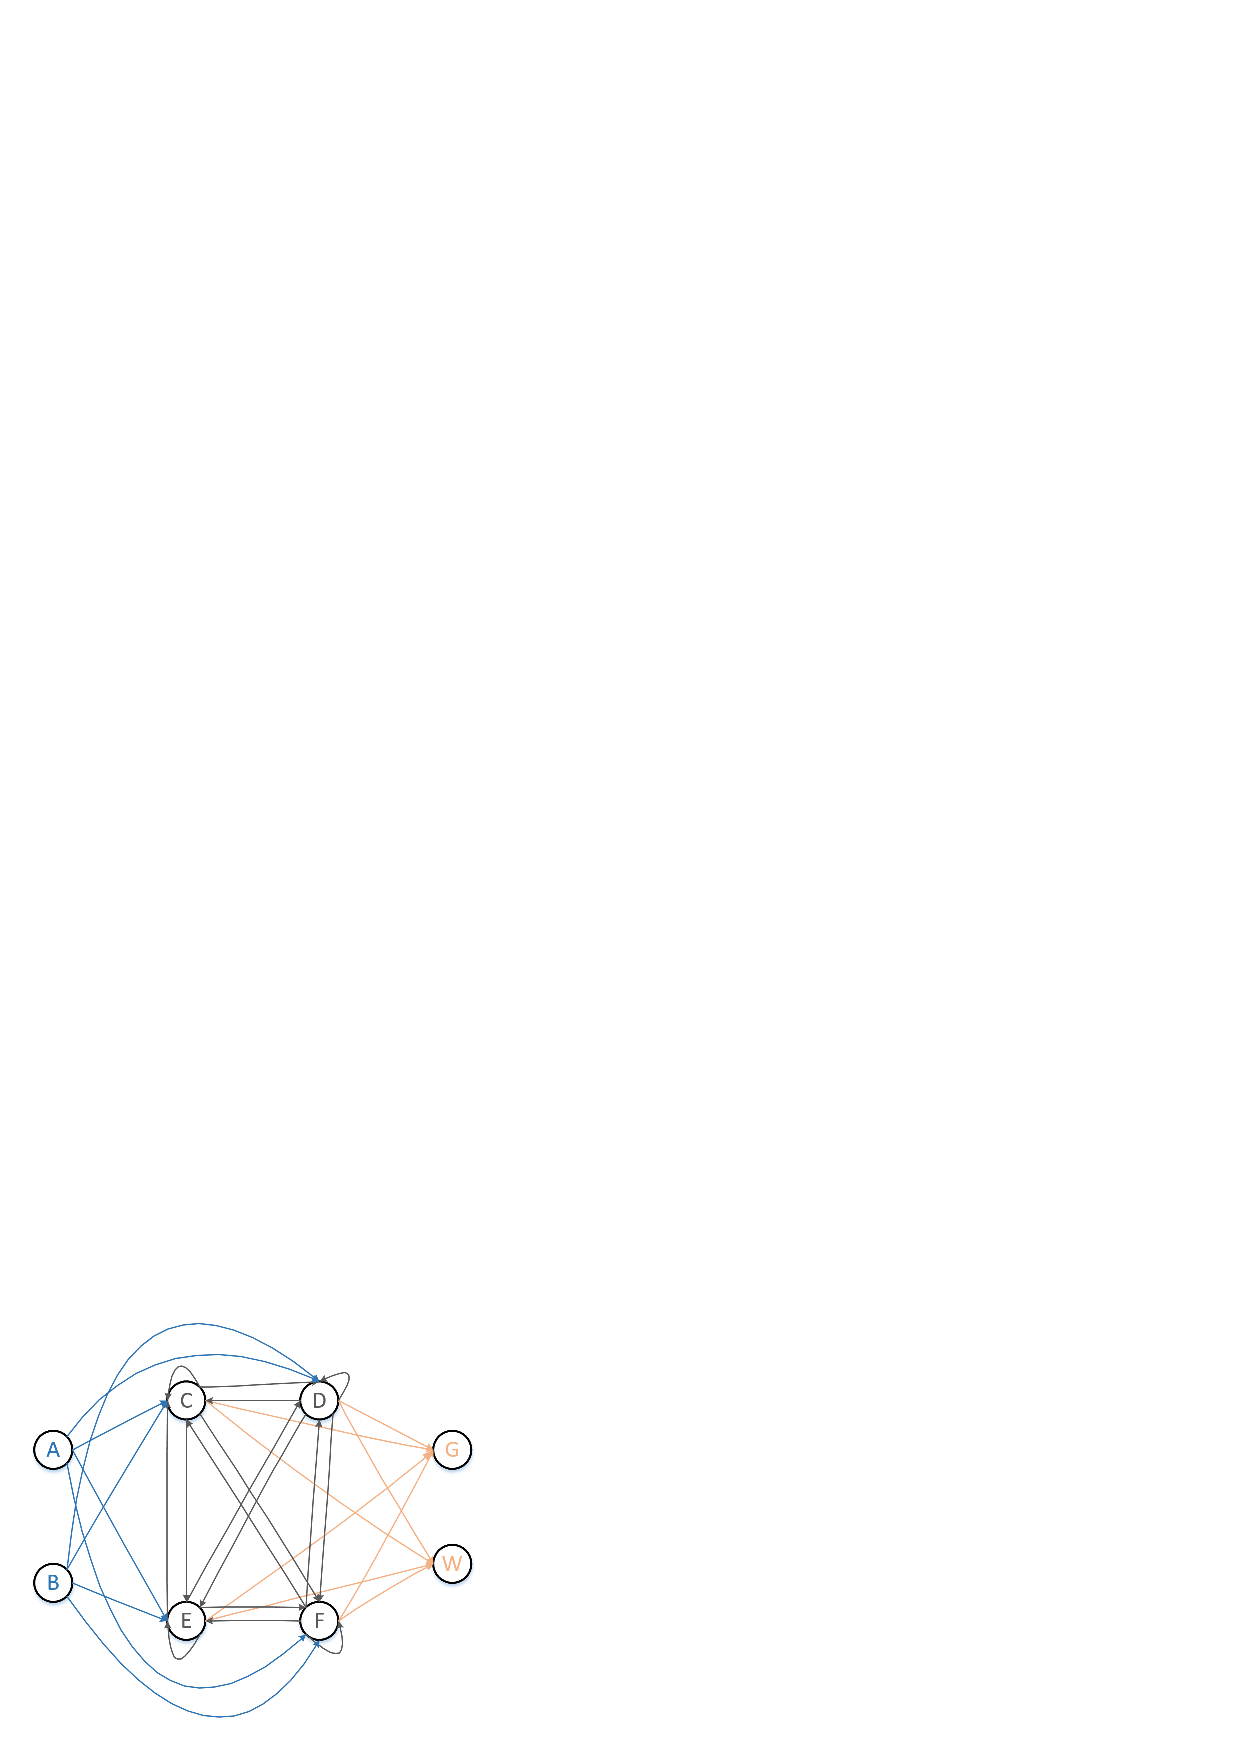
\includegraphics[scale=0.23]{figures/Fig1.png}}
		}}
		
		\caption{A Boolean control network. }%We use blue, black and orange, to distinguish three types of nodes and three types of edges. with two input-nodes $A$ and $B$, four state-nodes $C$, $D$, $E$ and $F$, and two output-nodes $G$, $W$.
		\label{fig:1}
	\end{figure}
%	
Let $\BB$ be the \BCN\  shown in Fig.~\ref{fig:1} which has two  input-nodes $I=\{\mathsf{i}_1,\mathsf{i}_2\}$ , four state-nodes $S=\{\mathsf{s}_1, \mathsf{s}_2,\mathsf{s}_3, \mathsf{s}_4\}$ and two output-nodes $O=\{\mathsf{o}_1,\mathsf{o}_2\}$. The set of edges $E$ and 
the updating rules $\sigma: \mathbb{B}^{2}\times \mathbb{B}^{4}\mapsto \mathbb{B}^4$ and $\rho:\mathbb{B}^4\mapsto \mathbb{B}^2$ are given in the truth table (Fig.~\ref{fig:2}) from which the updating rules in terms of logic functions can be easily recovered.   For instance, %from the truth table we have 
the updating rule of output-node $\mathsf{o}_1$ is 
$\mathsf{o}_1(t)=\mathsf{s}_1(t)\vee {({\mathsf{s}_2}(t)\wedge { \mathsf{s}_3}(t)\wedge {\mathsf{s}_4}(t))}$. 
%The set of all possible inputs $\mathcal{I}_\BB=\{\delta_{4}^0,\ldots,\delta_{4}^{3}\}$, the set of all states $\mathcal{S}_\BB=\{\delta_{16}^0,\ldots,\delta_{16}^{15}\}$ and the set of all outputs $\mathcal{O}_\BB=\{\delta_{4}^0,\ldots,\delta_{4}^{3}\}$.
 \begin{figure}[thpb]
	\centering
	\framebox{\parbox{3in}{
			\centerline{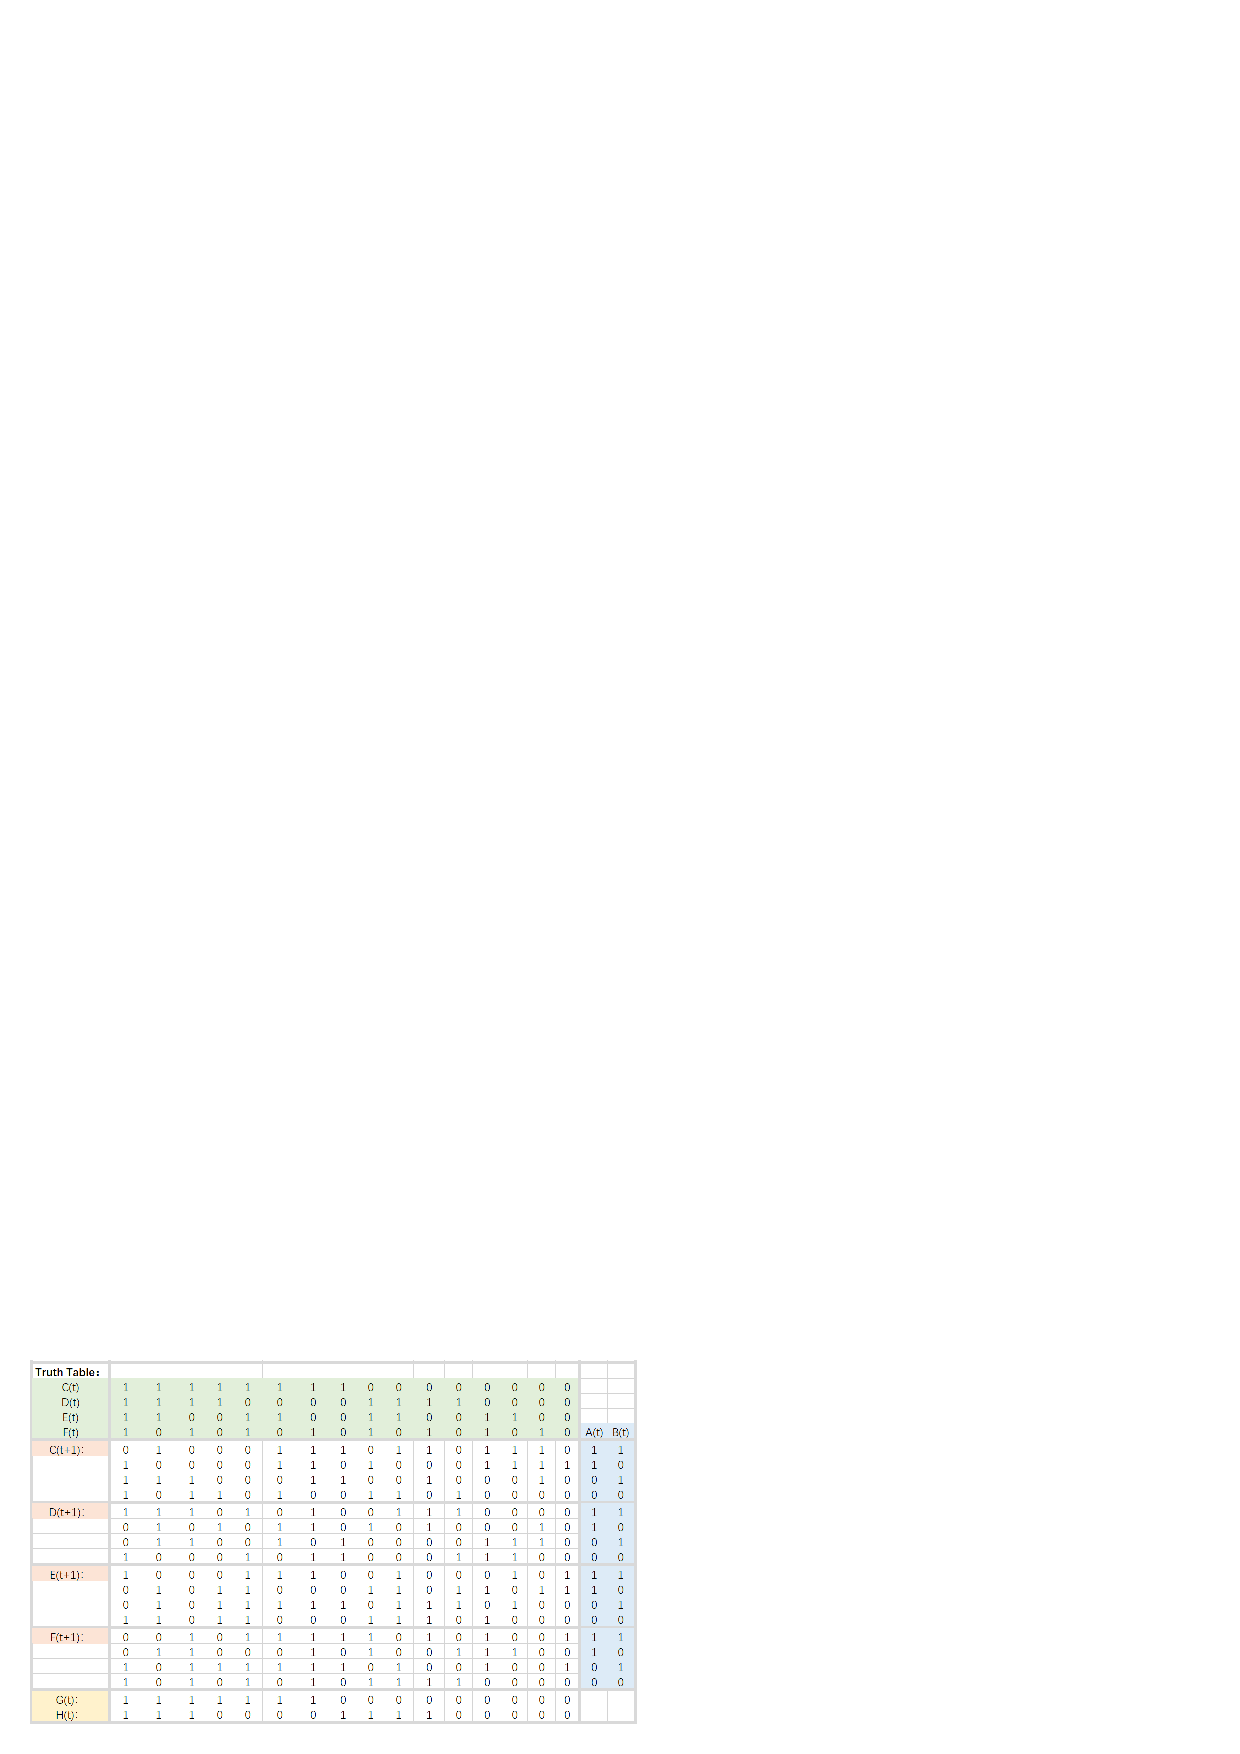
\includegraphics[scale=0.343]{figures/Fig2.png}}
	}}
	\caption{The truth table which describe the updating rules of the \BCN\ shown in Fig.~\ref{fig:1}.}
	\label{fig:2}
\end{figure}
%For instance, from the truth table we have the updating rule of output-node $G$ is 
%$G(t)=C(t)\vee {({D}(t)\wedge { E}(t)\wedge {F}(t))}.$
 %
\end{example}   

%===========================================================

%The reason why we use the truth table to describe the updating rules of the \BCN\ is that it would be more convenient for us to convert the $\mathsf{i}(t)$, $\mathsf{s}(t)$ and $\mathsf{o}(t)$ into their abbreviation forms. 
%That we use 
%\begin{itemize}
%  \item $\delta^i_{2^m}$ represents the abbreviation form of $\mathsf{i}(t)$, where $i=\sum_{x=1}^m \mathsf{i}_{x}(t)\times 2^{m-x}$;
%  \item $\delta^j_{2^n}$ represents the abbreviation form of $\mathsf{s}(t)$, where $j=\sum_{x=1}^n \mathsf{s}_{x}(t)\times 2^{n-x}$;
%  \item $\delta^w_{2^q}$ represents the abbreviation form of $\mathsf{o}(t)$, where  $w=\sum_{x=1}^q \mathsf{o}_{x}(t)\times 2^{q-x}$.
%\end{itemize}
%
%For instance if $\mathsf{s}(t)=\begin{bmatrix}\mathsf{s}_1(t)\\\mathsf{s}_2(t) \\ \mathsf{s}_3(t) \\\mathsf{s}_4(t)\end{bmatrix}=\begin{bmatrix}0\\1\\0\\1\end{bmatrix}$, then $\mathsf{s}(t)$ can be represented by $\delta^{(0\times2^3+1\times2^2+0\times2^1+1\times2^0)}_{2^4}=\delta^5_{16}$. 
%
%In the \BCN\ which shown in the Fig.~\ref{fig:1}, we consider 
%\begin{itemize}
%  \item $A(t)$ as $\mathsf{i}_{1}(t)$, $B(t)$ as $\mathsf{i}_{2}(t)$;
%  \item $C(t)$ as $\mathsf{s}_{1}(t)$, $D(t)$ as $\mathsf{s}_{2}(t)$;
%  \item $E(t)$ as $\mathsf{s}_{3}(t)$, $F(t)$ as $\mathsf{s}_{4}(t)$;
%  \item $G(t)$ as $\mathsf{o}_{1}(t)$, $W(t)$ as $\mathsf{o}_{2}(t)$.
%\end{itemize}
%
%Then, the updating rules which shown in Fig.~\ref{fig:2} can be represented by Fig.~\ref{fig:6}.
% \begin{figure}[thpb]
%      \centering
%      \framebox{\parbox{3in}{
%		\centerline{\includegraphics[scale=0.122]{figures/Fig7.png}}
%	}}
%      
%      \caption{The abbreviation form of the updating rules.}
%      \label{fig:6}
%   \end{figure}
%  
%   With the abbreviation forms of $\mathsf{i}(t)$, $\mathsf{s}(t)$ and $\mathsf{o}(t)$, it would be easier for us to use this \BCN\ to explain various concepts by checking this table.
  % 
%For instance, if $\mathsf{s}(t)=\delta^5_{16}$ and $\mathsf{i}(t)=\delta^1_{4}$, then we can know that $\mathsf{s}(t+1)=\delta^4_{16}$  and $\mathsf{s}(t+1)=\delta^1_{4}$ by checking this table.   
 % \tl{(1)simplify later?!} 
%   \begin{itemize}
% \item $\Delta_M = \{\delta^0_{2^m},\ldots,\delta^{({2^m}-1)}_{2^m} \}$ represents the input set; 
% \item $\Delta_N = \{\delta^0_{2^n},\ldots,\delta^{({2^n}-1)}_{2^n} \}$ represents the state set; 
% \item $\Delta_Q = \{\delta^0_{2^q},\ldots,\delta^{({2^q}-1)}_{2^q} \}$ represents the output set,
%\end{itemize}
%where $M=2^m$, $N=2^n$ and $Q=2^q$.
%=======================================================================

%=======================================================================


\subsection{Control theoretical properties of \BCNs}
In this subsection, we introduce the notations controllability, observability and identifiability of {\BCNs} and their relations. 
In particular, we will give a summary about the existing work on observability in order to motivate our work. To this end, first define some notations below.

Given a {\BCN} $\BB = (I,S,O, E, \sigma, \rho,\theta)$, let $\mathcal{I}$, $\mathcal{S}$ and $\mathcal{O}$ be the sets of all possible inputs, states and outputs of $\BB$, respectively. For any $t,t' \in \mathbb{T}$, we define the timed behavior of $\BB$
\begin{itemize}
\item $\mathcal{B}^T = (\mathcal{I}^T, \mathcal{S}^T, \mathcal{O}^T)$,  where 
{\small \[\begin{array}{llll}
\mathcal{I}^T =\{\mathsf{I}[t]~|~ t\in \mathbb{T}, \mathsf{I}[t]=\mathsf{i}(0)\ldots \mathsf{i}(t)\}\\
\mathcal{S}^T =\{\mathsf{S}[t]~|~ t\in \mathbb{T}, \mathsf{S}[t]=\mathsf{s}(0)\ldots \mathsf{s}(t)\}\\
\mathcal{O}^T =\{\mathsf{O}[t]~|~ t\in \mathbb{T}, \mathsf{O}[t]=\mathsf{o}(0)\ldots \mathsf{o}(t)\}\\
\end{array}
\]} such that each for any $\mathsf{s}(k)$ and $\mathsf{o}(k)$ of any $\mathsf{S}[t]$ and 
$\mathsf{O}[t]$ in $\mathcal{S}^T$ and $\mathcal{O}^T$, respectively,   satisfies the updating rules in Definition~\ref{def:BCN}.
\item Let $\mathsf{S}(t) = \{ s(t)~|~ s(0)\ldots s(t) \in \mathcal{S}^T\}$ and $\mathsf{O}(t) = \{ o(t)~|~ o(0)\ldots o(t) \in \mathcal{O}^T\}$, which do not necessarily have all the possible $2^m$ and $2^n$ as they are generated in the timed behavior according to the updating rules. Note that at any time the input node can take any value in $\mathbb{B}$.
\item For any interval  $[t_0,t]$ of time $\mathbb{T}$, where $t\geq t_0$, we define the following sets 
\[\begin{array}{llllll}
\mathcal{I}^{[t]} &=& \{\mathsf{I}[t] ~|~ \mathsf{I}[t]\in \mathcal{I}^T\}\\
\mathcal{I}^{[t_0,t]} &=& \{\mathsf{i}(t_0)\ldots \mathsf{i}(t)~|\exists \mathsf{i}(0)\ldots \mathsf{i}(t)\in \mathsf{I}^{[t_0]}\cdot\\
&& \mathsf{i}(0)\ldots \mathsf{i}(t_0) \ldots \mathsf{i}(t)\in \mathcal{I}^{[t]} \\
\mathcal{S}^{[t]} &=& \{\mathsf{S}[t] ~|~ \mathsf{S}[t]\in \mathcal{S}^T\}\\
\mathcal{S}^{[t_0,t]} &=& \{\mathsf{s}(t_0)\ldots \mathsf{s}(t+1)~|\exists \mathsf{s}(0)\ldots \mathsf{s}(t_0)\in \mathcal{S}^{[t_0]}\cdot\\
&& \mathsf{s}(0)\ldots \mathsf{s}(t_0) \ldots \mathsf{s}(t+1)\in \mathcal{S}^{[t+1]} \\
\mathcal{O}^{[t]} &=& \{\mathsf{O}[t] ~|~ \mathsf{O}[t]\in \mathcal{O}^T\}\\
\mathcal{O}^{[t_0,t]} &=& \{\mathsf{o}(t)\ldots \mathsf{o}(t_0)~|\exists \mathsf{o}(0)\ldots \mathsf{o}(t_o)\in \mathcal{O}^{[t_0]}\cdot\\
&& \mathsf{o}(0)\ldots \mathsf{o}(t_o) \ldots \mathsf{o}(t+1)\in \mathcal{O}^{[t+1]} \\
\end{array}
\]
\end{itemize} 
The sets $\mathcal{I}^{[t_0,t]}$, $\mathcal{S}^{[t_0,t]}$ and $\mathcal{O}^{[t_0,t]}$ are the possible inputs, states and outputs of the execution of $\BB$ in the interval $[t_0,t]$ of observing time. 

		We now define the following two functions which define,  for any interval $[t_0,t]$ of observing time from $t_0$ to $t$,  the sequence of states and sequence of outputs produced, respectively,  in the interval by a state $\mathsf{s}(t_0)$ at time $t_0$ and a sequence of inputs in the interval. Formally, the two functions are defined as:


\begin{equation}
\begin{split}
F^{[t_0,t]}&: S(t_0)\times \mathcal{I}^{[t_0,t]} \mapsto \mathcal{S}^{[t_0,t+1]}\\
F^{[t_0,t]}&(\mathsf{s}, \mathsf{i}(t_0)\ldots \mathsf{i}(t))= \mathsf{s}(t_0+1)\ldots \mathsf{s}(t+1)\\
 \end{split}
\end{equation}
 \begin{equation}
\begin{split}
 H^{[t_0,t]}&: S(t_0)\times \mathcal{I}^{[t_0,t]} \mapsto \mathcal{O}^{[t_0,t+1]}\\
H^{[t_0,t]}&(\mathsf{s}, \mathsf{i}(t_0)\ldots \mathsf{i}(t))= \mathsf{o}(t_0+1)\ldots \mathsf{o}(t+1)\\
\end{split}
\end{equation}

\[
\begin{array}{llllll}
\mbox{such that the following conditions are satisfied}\\
 (\mathsf{s}(t_0)=\mathsf{s})\wedge \\
 \forall t'=(t_0+1),\ldots,(t+1)\cdot (\mathsf{s}(t')=\sigma(\mathsf{i}(t'-1),\mathsf{s}(t'-1)))\wedge \\
 \forall t'=t_0,\ldots,(t+1)\cdot (\mathsf{o}(t')=\rho(\mathsf{s}(t'))
\end{array}
\]

These functions generalize the two functions given in ~\cite{Zhang2016Observability} for observability,  where only the special case of $F^{[0,t]}$ and $H^{[0,t]}$ are given. The their extensions  will be used when we present the the new observability.
\begin{definition} [Observability~\cite{cheng2009controllability, Zhao2010Input, Cheng2011Identification, Fornasini2013Observability}]
We define the four types of observability below. 
\begin{itemize}
  \item The {\bf Type-I} observability is that, a \BCN\ is observable if for every initial state \State$(0)\in \mathcal{S}$, there exists an input sequence $\mathsf{I}[t]\in\mathcal{I}^{[t]}$ for some $t>0$, such that for all states $\mathsf{s}'(0)\neq \mathsf{s}(0)$, $H^{[0,t]}(\mathsf{s}'(0),\mathsf{I}[t])\neq H^{[0,t]}(\mathsf{s}(0), \mathsf{I}[t])$.
  \item The  {\bf Type-II} observability is that, a \BCN\ is observable if for every two distinct initial states $\mathsf{s}(0)$, $\mathsf{s}'(0) \in \mathcal{S}$, there is an input sequence $\mathsf{I}[t]\in\mathcal{I}^{[t]}$ for some $k>0$, such that $H^{[0,t]}(\mathsf{s}'(0),\mathsf{I}[t])\neq H^{[0,t]}(\mathsf{s}(0), \mathsf{I}[t])$.
  \item The {\bf Type-III} observability is that, a \BCN\ is observable if there exists an input sequence $\mathsf{I}[t]\in\mathcal{I}^{[t]}$ for some $t>0$, such that for any two distinct states $\mathsf{s}(0)$, $\mathsf{s}'(0) \in \mathcal{S}$, $H^{[0,t]}(\mathsf{s}'(0),\mathsf{I}[t])\neq H^{[0,t]}(\mathsf{s}(0), \mathsf{I}[t])$.
  \item The {\bf Type-IV} observability is that, a \BCN\ is observable, if there is a  natural number $N$, such that for every input sequence $\mathsf{I}[t]\in\mathcal{I}^{[t]}$, for any two distinct states $\mathsf{s}(0)$, $\mathsf{s}'(0) \in \mathcal{S}$, $H^{[0,t]}(\mathsf{s}'(0),\mathsf{I}[t])\neq H^{[0,t]}(\mathsf{s}(0), \mathsf{I}[t])$ if  $t\ge N$.
\end{itemize} 
\end{definition}

%The  {\bf Type-I} observability means that a \BCN\ is observable if every \State$(0)$ of the \BCN\ can be distinguished from other types of initial state by an input sequence $\mathsf{I}[k]$. The {\bf Type-II} observability means that a \BCN\ is observable if for every two distinct $\mathsf{s}(0)$, $\mathsf{s}'(0)$, there is an input sequence $\mathsf{I}[k]$ which distinguishes them.
 %The {\bf Type-III} observability means that a \BCN\ is called observable if there exists an input sequence $\mathsf{I}[k]$ which determine the $\mathsf{s}(0)$ of the \BCN\ for every $\mathsf{s}(0)\in\mathcal{S}$, because $\mathsf{I}[k]$ can distinguish all distinct initial states. The {\bf Type-IV} observability means that a \BCN\ is observable if every sufficient long $\mathsf{I}[k]$ can determine the $\mathsf{s}(0)$ of the \BCN\ for every $\mathsf{s}(0)\in\mathcal{S}$.


 %Thus, we can only check whether $\mathsf{s}(0)=\mathsf{s}^{x}(0)$ or not by $\mathsf{I}^x$. %
%\begin{example}
%For example, for the \BCN\ mentioned in {\em Example \ref{exa:2}}, we have every \State$(0)$ can be distinguished from other types of initial state by an $\mathsf{I}[k] \in(\mathcal{I})^k$.  For instance,
%\begin{itemize}
%  \item $\delta_{16}^0$ can be distinguished from other types of initial state by any $\mathsf{I}[k]$ with the prefix $\delta_{4}^3$, $\delta_{4}^2$ or $\delta_{4}^0  \delta_{4}^2$;%
%  \item $\delta_{16}^1$ can be distinguished from other types of initial state by any $\mathsf{I}[k]$ with the prefix $\delta_{4}^0$, $\delta_{4}^3$ or $\delta_{4}^2 \delta_{4}^3$;
 % \item $\delta_{16}^2$ can be distinguished from other types of initial state by any $\mathsf{I}[k]$ with the prefix $\delta_{4}^1$, $\delta_{4}^3$ or $\delta_{4}^0 \delta_{4}^2$, etc.
%\end{itemize} 
%Therefore, this \BCN\ satisfies the  {\bf Type-I} observability.
%\label{exa:4}
%\end{example}   

%\begin{definition}[ {\bf Type-II} Observability~\cite{Zhao2010Input}]
%	The  {\bf Type-II} observability is that, a \BCN\ is observable if for every two distinct initial states $\mathsf{s}(0)$, $\mathsf{s}'(0) \in \mathcal{S}$, there is an input sequence $\mathsf{I}[k]\in(\mathcal{I})^k$ for some $k>0$, such that $\rho(\mathsf{s}(0))=\rho(\mathsf{s}'(0))$ implies $(HF)^k_{\mathsf{s}(0)}(\mathsf{I}[k])\neq (HF)^k_{\mathsf{s}'(0)}(\mathsf{I}[k])$.
%\end{definition}

 %Therfore, we can only check $\mathsf{s}(0)=\mathsf{s}^{x}(0)$ or $\mathsf{s}(0)=\mathsf{s}^{y}(0)$ when we know that $\mathsf{s}(0)$ is one of them by $\mathsf{I}^{xy}$. 
%\begin{example}
%For example, for the \BCN\ mentioned in {\em Example \ref{exa:2}}, we have for every two distinct $\mathsf{s}(0)$ and $\mathsf{s}'(0)$, there exists an $\mathsf{I}[k]\in(\mathcal{I})^k$ which distinguishes them.  For instance,
%\begin{itemize}
 % \item $\mathsf{I}[k]$ with the prefix $\delta_{4}^0$ can distinguish $\delta_{16}^0$ and $\delta_{16}^1$;
 % \item $\mathsf{I}[k]$ with the prefix $\delta_{4}^1$ can distinguish $\delta_{16}^0$ and $\delta_{16}^2$;
 % \item $\mathsf{I}[k]$ with the prefix $\delta_{4}^3$ can distinguish $\delta_{16}^1$ and $\delta_{16}^2$.
%\end{itemize} 
%Therefore this \BCN\ satisfies the {\bf Type-II} observability.
%\label{exa:5}
%\end{example}   
%\begin{definition}[{\bf Type-III} Observability~\cite{Cheng2011Identification}]
%The {\bf Type-III} observability is that, a \BCN\ is observable if there exists an input sequence $\mathsf{I}[k]\in(\mathcal{I})^k$ for some $k>0$, such that for any two distinct states $\mathsf{s}(0)$, $\mathsf{s}'(0) \in \mathcal{S}$, $\rho(\mathsf{s}(0))=\rho(\mathsf{s}'(0))$ implies $(HF)^k_{\mathsf{s}(0)}(\mathsf{I}[k])\neq (HF)^k_{\mathsf{s}'(0)}(\mathsf{I}[k])$.
%\end{definition}

%, the $\mathsf{s}(0)$ is determined by its corresponding output sequence $(HF)^k_{\mathsf{s}(0)}(\mathsf{I})$.

%\begin{example}
%For example, for the \BCN\ mentioned in {\em Example \ref{exa:2}}, for any $k>0$, there is not an $\mathsf{I}[k]\in(\mathcal{I})^k$ which determines the $\mathsf{s}(0)$ of this \BCN:
%\begin{itemize}
 % \item $\mathsf{I}[k]$ with prefix $\delta_{4}^0$ can not distinguish $\delta_{16}^9$ and $\delta_{16}^{10}$;
%  \item $\mathsf{I}[k]$ with prefix $\delta_{4}^1$ can not distinguish $\delta_{16}^0$ and $\delta_{16}^{1}$;
%  \item $\mathsf{I}[k]$ with prefix $\delta_{4}^2$ can not distinguish $\delta_{16}^3$ and $\delta_{16}^{4}$;
 % \item $\mathsf{I}[k]$ with prefix $\delta_{4}^3$ can not distinguish $\delta_{16}^{14}$ and $\delta_{16}^{15}$.
%\end{itemize} 
%Therefore it does not satisfy the {\bf Type-III} observability. 
%\label{exa:6}
%\end{example}  
%\begin{definition}[{\bf Type-IV} Observability~\cite{Fornasini2013Observability}]
%	The {\bf Type-IV} observability is that, a \BCN\ is observable, if there is a  natural number $N$, such that for every input sequence $\mathsf{I}[k]\in(\mathcal{I})^{k}$, for any two distinct states $\mathsf{s}(0)$, $\mathsf{s}'(0) \in \mathcal{S}$, $\rho(\mathsf{s}(0))=\rho(\mathsf{s}'(0))$ implies $(HF)^{k}_{\mathsf{s}(0)}(\mathsf{I}[k])\neq (HF)^{k}_{\mathsf{s}'(0)}(\mathsf{I}[k])$ if  $k\ge N$.
%\end{definition}

%, because every sufficient long $\mathsf{I}[k]$ can distinguish any two distinct initial states.%, the $\mathsf{I}$ can be determined by its output sequence $(HF)^k_{\mathsf{s}(0)}(\mathsf{I})$.
%\begin{example}
%For example, for the \BCN\ mentioned in {\em Example \ref{exa:2}}, any $\mathsf{I}[k]$ with prefix $\delta_{4}^0$ can not can not distinguish $\delta_{16}^9$ and $\delta_{16}^{10}$. 
%Therefore this \BCN\ does not satisfy the {\bf Type-IV} observability. 
%\label{exa:7}
%\end{example}  

The implication relationships of four existing types of observability is that, {\bf Type-I} observability is stronger than {\bf Type-II} observability, {\bf Type-III} observability is stronger than {\bf Type-I} observability and {\bf Type-II} observability, while {\bf Type-IV} observability is strongest~\cite{Zhang2016Observability}. If a \BCN\ satisfies {\bf Type-I} observability, then for every initial state $\mathsf{s}(0)$ there exists an input sequence $\mathsf{I}[k]$ which can distinguish $\mathsf{s}(0)$ from other initial states, and then in this \BCN, for every two distinct initial states $\mathsf{s}(0)$, $\mathsf{s}'(0) $ there exists an input sequence $\mathsf{I}'[k]$ which can distinguish them, thus it satisfies {\bf Type-II} observability. Therefore, {\bf Type-I} observability is stronger than {\bf Type-II} observability. If a \BCN\ satisfies {\bf Type-III} observability, then there exists an input sequence $\mathsf{I}[k]$ which can distinguish every two distinct initial states $\mathsf{s}(0)$, $\mathsf{s}'(0)$, and then in this \BCN, for every initial state $\mathsf{s}(0)$ the input sequence $\mathsf{I}[k]$ can distinguish $\mathsf{s}(0)$ from other initial states, thus it satisfies {\bf Type-II} observability. Therefore, {\bf Type-III} observability is stronger than {\bf Type-I} observability and {\bf Type-II} observability. If a \BCN\ satisfies {\bf Type-IV} observability, then every sufficient long input sequence $\mathsf{I}[k]$ can distinguish every two distinct initial states $\mathsf{s}(0)$, $\mathsf{s}'(0)$, thus it satisfies {\bf Type-III} observability too. Therefore, {\bf Type-IV} observability is strongest. 

% \begin{figure}[thpb]
   %  \centering
 %   \framebox{\parbox{3in}{
%		\centerline{\includegraphics[scale=0.27]{figures/Fig9.png}}
%	}}
      
   %  \caption{The implication relationships graph between observability {\bf Type-I}, {\bf Type-II}, {\bf Type-III} and {\bf Type-IV}, where ``$\rightarrow$" means ``implies".}
%      \label{fig:9}
  % \end{figure}

%The implication relationship is that ``The first observability implies the second observability.'' means ``If a \BCN\ satisfies the first observability, then it satisfies the second observability.'' 



%\subsection{Controllability and identifiability of \BCNs}
%\tl{what's the point here?}


\begin{definition}[Controllability~\cite{cheng2009controllability}]
	A \BCN\ is controllable if for any two distinct states $\mathsf{s}$, $\mathsf{s}' \in \mathcal{S}$, there is an input sequence $\mathsf{I}[k]\in(\mathcal{I})^k$ for some $k>0$, such that in the  $F^k_{\mathsf{s}(0)}(\mathsf{I}[k])=\mathsf{s}(1) \ldots\, \mathsf{s}(k)$, the $\mathsf{s}(0)=\mathsf{s}$ and $\mathsf{s}(k)=\mathsf{s}'$.
\end{definition}

%\begin{example}
%For example, the \BCN\ mentioned in {\em Example \ref{exa:2}} is controllable, that is for any initial state $\mathsf{s}(0)$ and destination state $\mathsf{s}'$, there is an input sequence $\mathsf{I}[k]$, such that in the $F^k_{\mathsf{s}(0)}(\mathsf{I}[k])=\mathsf{s}(1) \ldots\, \mathsf{s}(k)$, the $\mathsf{s}(k)=\mathsf{s}'$. For instance, for the initial state $\mathsf{s}(0)= \delta_{16}^{1}$ and destination state $\mathsf{s}'=\delta_{16}^{2}$, there is an input sequence $\mathsf{I}[3]=\delta_{4}^{3}\delta_{4}^{3}\delta_{4}^{3}$, such that $F^3_{\mathsf{s}(0)}(\delta_{4}^{3}\delta_{4}^{3}\delta_{4}^{3})=\delta_{16}^{13}\delta_{16}^{11}\delta_{16}^{2}$.
%\label{exa:12}
%\end{example}  

\begin{definition}[Identifiability~\cite{Cheng2011Identification}]%
	A \BCN\ is identifiable if there exists an input sequence $\mathsf{I}[k]\in(\mathcal{I})^k$ for some $k>0$, such that the updating rules
	\begin{equation*}
    		\begin{split}
		\mathsf{s}(t+1)=&\sigma(\mathsf{i}(t),\mathsf{s}(t))\\
		\mathsf{o}(t)=&\rho(\mathsf{s}(t))
		\end{split}
	\end{equation*}
	can be determined by $\mathsf{I}[k]$ and $H^k_{\mathsf{s}(0)}(\mathsf{I}[k])$.
\end{definition}

%\begin{definition}[Observability]
%A \BCN\ $\BB$ is observable if there exists an input sequence $\mathsf{I}\in(\Delta_L)^k$ for some $k>0$, such that for any two distinct states $\mathsf{s}(0)$, $\mathsf{s}'(0) \in \Delta_M$, $h(\mathsf{s}(0))=h(\mathsf{s}'(0))$ implies $(HF)^k_{\mathsf{s}(0)}(\mathsf{I})\neq (HF)^k_{\mathsf{s}'(0)}(\mathsf{I})$ \cite{Cheng2011Identification}.
%\end{definition}

%The observability means that a \BCN\ is called observable if there exists an input sequence $\mathsf{I}\in(\Delta_L)^k$ which determine the $\mathsf{s}(0)$ of the \BCN\ for every $\mathsf{s}(0)\in\Delta_M$, because $\mathsf{I}$ can distinguish any two distinct initial states.%, the $\mathsf{s}(0)$ is determined by its corresponding output sequence $(HF)^k_{\mathsf{s}(0)}(\mathsf{I})$.

%\begin{example}
%For example, for the \BCN\ mentioned in {\em Example \ref{exa:2}}, for any $k>0$, there is not any $\mathsf{I}\in(\Delta_L)^k$ which can determine the $\mathsf{s}(0)$ of this \BCN:
%\begin{itemize}
 % \item any $\mathsf{I}$ with prefix $\delta_{4}^0$ can not distinguish $\delta_{16}^9$ and $\delta_{16}^{10}$;
 % \item any $\mathsf{I}$ with prefix $\delta_{4}^1$ can not distinguish $\delta_{16}^0$ and $\delta_{16}^{1}$;
  %\item any $\mathsf{I}$ with prefix $\delta_{4}^2$ can not distinguish $\delta_{16}^3$ and $\delta_{16}^{4}$;
%  \item any $\mathsf{I}$ with prefix $\delta_{4}^3$ can not distinguish $\delta_{16}^{14}$ and $\delta_{16}^{15}$.
%\end{itemize} 
%Therefore it does not satisfy the observability. 
%\label{exa:6}
%\end{example}  

A \BCN\ $\BB$ is identifiable iff $\BB$ is controllable and $\BB$'s initial state $\mathsf{s}(0)$ can be determined  without  resetting~\cite{Cheng2011Identification}. And in \cite{Cheng2011Identification}, the authors regard the {\bf Type-III} observability as the necessary and sufficient condition of determining the initial state $\mathsf{s}(0)$  without  resetting. But we discover that the  {\bf Type-III} observability is sufficient but not necessary condition. Thus, we propose the online observability to present the necessary and sufficient condition.
%, because the initial state $\mathsf{s}(0)$ of a \BCN\ $\BB$ can be determined by the algorithm (mentioned in {\em Section \ref{sec:intro}}) corresponding to {\bf Type-III} observability when $\BB$ satisfies the {\bf Type-III} observability.


   
% Because we do not make full use of the output and input in the process of determining the initial state. The output of \BCNs\ we observe at every time step can help us further determine the range of the initial state. With the range of the initial state, we can use different input sequence to determine the initial state. While in the third and fourth existing observability, we use the same input sequence $\mathsf{I}$ to determine the initial state.

 
%However, in some biological systems which depicted by \BCNs, the initial states of them can be checked at most once. Therefore,
%The {\bf Type-I} observability and {\bf Type-II} observability are designed to determine the initial states of \BCNs\ when their initial state can be reset. The {\bf Type-IV} observability is designed to study the reconstructibility of \BCN. The {\bf type-III} observability is proposed to research the identification of \BCNs. In this paper, we want to use the new observability we propose to replace the {\bf Type-III} observability, such that we can research the identification problem better.
%As the first observability and second observability are designed to determine the initial states of \BCNs\ by taking the determining procedure multiple times in parallel. %\tl{why this claim?} 
%And in some applications, we have to determine \BCNs' initial states by taking the determining procedure once. The third and fourth observability are designed to determine the initial states of \BCNs\ by taking the determining procedure once. But if a \BCN\ is not satisfy the third observability, we can not use them to determine its initial states by taking the determining procedure once.  %Thus, we propose the online observability of \BCNs\ to solve the problem.
%Moreover, in some biological systems, it would takes many costs to check these biological systems. Hence it would cost a lot of overhead for us to determine the initial state of them by the first observability and second observability.





% \begin{problem}
%\label{pro:2}
%What is the necessary and sufficient condition of determining a \BCN's initial state $\mathsf{s}(0)$ by taking the determining procedure once?
%\end{problem}


% !Mode\dots ``TeX:UTF-8''
% !TEX root = ../root.tex
\section{The online observability of \BCNs}
\label{sec:online}
In this section we propose the online observability. We give the informal definition of it at first. 

%\begin{definition}
	A \BCN\ has online observability, if every initial state $s_0 \in \Delta_N$ can be determined in real time. In the online observability we determine the state of \BCN\ by dynamically deciding input sequence and observing output sequence at every time step. And this process can be accomplished in finite time steps.
%\end{definition}  without presupposing the initial state of \BCN

The reason why we called this kind of observability online observability is that:
\begin{itemize}
  \item In this kind of observability, we determine the initial state of \BCNs\ in real time. In other words, we can use one test case to determine the initial state of \BCNs. We call this property {\em real-time} property.%Such that we can determine the initial state of any test case of \BCNs.
  \item In online observability, we use the outputs we observe to adjust the input sequence at every time step. By this way, we can make full use of the outputs to determine the initial state of \BCNs. We call this property {\em interactivity}.
\end{itemize} 

We can determine the initial state of any test case of a \BCN\ when we can use one test case to determine the initial state of it. We need {\em real-time} property to help us avoid repeating biological experiments. And the {\em interactivity} would help us to find the necessary and sufficient condition of determine the initial state of \BCNs\ in real time. With the  {\em real-time} and {\em interactivity}, we called this kind of observability online observability.
%\tl{maybe I did not understand this, but I think you are confusing two things: the observability and the algorithm (approach) to determine the initial state. It seems to me that you are describing a new approach (the online approach), but does this change the observability? if yes, how? Is this a stronger notion or a weaker notion or incomparable?}

In the left of this section, firstly we present the definition of deduction function. Secondly we present the definition of $K$ steps determinability. We take them as the preparations for defining the online observability. Finally, we give the formal definition of the online observability of \BCNs. 
\subsection{Deduction function}
%Different from four existing observabilities, t
The observability we propose can determine the initial state online.
 %Because in the process of determining the initial state every input of the input sequence is decided by the output we observe at every time step. 
 In the time setp $k$, we observe the output of \BCNs\ at first. Through this we can infer the possible values of state-nodes and denote them by possible states set $S_k$. %Then as we can know the possible states set, 
 At the next step, we need to decide the input $i_k$ which satisfies that % will make sure any different possible states 
$s_i, s_j$ 
 will not turn into the same state after being affected by the input $i_k$ i.e., $Ls_i i_k\neq Ls_j i_k$ for any distinct $s_i, s_j\in S_k$. After deciding input, we can observe the new output, and then we can infer the new possible states set. The cardinal number of possible states set after we inputted will not lager than the cardinal number of possible states set before we input. If the cardinal number of possible states set turn into be $1$ then we can determine the state and the initial state of {\em BCN}. And the reason why the cardinal number of the possible states set would decrease is shown in equation (\ref{equ:10}) and (\ref{equ:11}). 
 
To better describe the deduction process of \BCN\ initial state we mentioned before, we give a deduction function for it. The definition of this function is as follows.
\begin{definition}[Deduction Function] The deduction function can be defined as $\Ded\left(S, i, o\right)$. Using this function we can get a states set $\Ded\left(S, i, o\right)$ for $S$ after inputing $i$ and observing $o$. Therefore, based on deduction process mentioned before, we have that there exists the corresponding $s(t)\in S$ of $s(t+1)$ such that \[s(t+1)=L\ltimes i\ltimes s(t)\ when\ i\neq \varepsilon, \] and \[H\ltimes s(t+1)=o\ when\ o\neq \varepsilon, \]
for each element \[s(t+1)\in \Ded\left(S, i, o\right)\]
\end{definition}
where   
\begin{itemize}
  \item $S\in 2^{\Delta_N}$ is the possible states set;
  \item $i\in (\Delta_M\cup\varepsilon)$ represents the input;
  \item $o\in(\Delta_Q\cup\varepsilon)$ represents the output; 
  \item $\Ded\left(S, i, o\right)\in 2^{\Delta_N}$ is the possible states set after deduction.
\end{itemize} 
 
 From the definition of deduction function, we have some equations for this function. By researching these equations, we can know the details of this function better.
\begin{equation}
\begin{split}
\Ded\left(\emptyset,i,o\right)=\emptyset\\
%D\left(\varnothing,I_i,O_i\right)=D\left(\varnothing,\varepsilon,O_i\right)= &D\left(\varnothing,\varepsilon,\varepsilon\right)=\varnothing\\
\end{split}
\label{equ:7}
\end{equation}

Equation (\ref{equ:7}) represents that if the possible states set is an empty set $\emptyset$ then no matter what we input and observe, we can only deduce the possible set is $\emptyset$. It means that if we don't know anything about the state of a \BCN, then we can not deduce anything no matter what we do.
\begin{equation}
\begin{split}
\Ded\left(S,\varepsilon,\varepsilon\right)=&S\\
\end{split}
\label{equ:8}
\end{equation}

For any possible states set $S$ and we neither input anything and nor observe the output. In this case we can only deduce that the possible states set is $S$ shown in equation (\ref{equ:8}). It means that before inputing and observing the output of \BCN\ we can not know more information about this \BCN\ than we used to knew.
\begin{equation}
\begin{split}
\Ded\left(\Delta_N,\varepsilon,\delta_4^1\right)=&\{\delta_{16}^1,\delta_{16}^2,\delta_{16}^3\}\\
\end{split}
\label{equ:9}
\end{equation}
 
 Using the example mentioned before (\ref{equ:4}), when the possible states set $S=\Delta_N$, and  we observe that the outputs of \BCN\ is $\delta_4^1$ before we decide input. In this case we can deduce that the possible states would be $\delta_{16}^1$, $\delta_{16}^2$ or  $\delta_{16}^3$ shown in equation (\ref{equ:9}).
\begin{equation}
\begin{split}
\Ded\left(\{\delta_{16}^1,\delta_{16}^2,\delta_{16}^3\},\delta_4^1,\varepsilon\right)=&\{\delta_{16}^{10},\delta_{16}^4,\delta_{16}^{11}\}\\
\end{split}
\label{equ:10}
\end{equation}

And then, if the possible states set $S=\{\delta_{16}^1$, $\delta_{16}^2$, $\delta_{16}^3\}$ we input $\delta_4^1$. Before we observe the output of \BCN\ we can only deduce the possible states would be $\delta_{16}^{10}$, $\delta_{16}^4$ or  $\delta_{16}^{11}$ shown in equation (\ref{equ:10}). In other words, the cardinal number of the possible states set did not decrease before observing the output of this \BCN.
\begin{equation}
\begin{split}
\Ded\left(\{\delta_{16}^1,\delta_{16}^2,\delta_{16}^3\},\delta_4^1,\delta_4^3\right)=&\{\delta_{16}^{10},\delta_{16}^{11}\}\\
\end{split}
\label{equ:11}
\end{equation}

But if we observe that the output of \BCN\ is $\delta_4^3$, then we can deduce that the possible state can be $\delta_{16}^{10}$ or  $\delta_{16}^{11}$ shown in equation (\ref{equ:11}). Such that the cardinal number of the possible states set may decrease after observing the output of \BCN.
\begin{equation}
\begin{split}
\Ded\left(\{\delta_{16}^4,\delta_{16}^5,\delta_{16}^6\},\delta_4^3,\varepsilon\right)=&\{\delta_{16}^9,\delta_{16}^{13}\}
\end{split}
\label{equ:12}
\end{equation}

 Finally if the set of possible states is $\{\delta_{16}^4,\delta_{16}^5,\delta_{16}^6\}$ and the inputs is $\delta_4^3$. Before we observe the output of \BCN\ we can deduce that the possible state values can be $\delta_{16}^9$ or $\delta_{16}^{13}$ shown in equation (\ref{equ:12}). Because both $\delta_{16}^4$ and $\delta_{16}^5$ are turn into be the same state $\delta_{16}^9$ after affected by $\delta_4^3$. And if the initial state of the \BCN\ is one of them then we can not determine the initial state any more. If the cardinality number of the possible states set of one \BCN\ decreased before observing its output the deduction process, then we can not deduce its initial state any more. 

\subsection{$k$-step determinability}
After we difined the deduction function, we can present the definition of $k$-step determinability of the states set of \BCNs\ and the range of $k$ is the set of natural numbers. It may easier to difine online observability by programming language. But we would like to define its mathematical form for preciseness of concepts. However, before defining the online observability of \BCNs, we need to difine the $k$-step determinability of the states set of \BCNs\ at first.
\begin{definition}[$k$-Step Determinability] 
When $k=0$, a set of states $S$ the $S$ is $0$-step deterministic if the cardinal number of this states set $|S|=1$. When $k>0$, a set of states $S$ is $k$-step deterministic
 if the cardinal number of this states set $|S|>1$, and for this set of states $S$ there exists $i_p$ in $\Delta_M$ such that
 \begin{itemize}
 \item  $|\Ded\left(S,i_p,\varepsilon\right)|=|S|, $ and 
 \item  for each $o_j$ in $\Delta_Q$ such that $|\Ded\left(S,i_p,o_j\right)|\neq 0$ and $\Ded\left(S,i_p,o_j\right)$ is $k'$-step deterministic with  ${k'}<k$.
 \end{itemize}
 And we default $k\ge0$ when we talk about whether a states set of \BCNs\ $S$ is $k$-step deterministic or not.
\end{definition}

From the definition of {\em$k$}-stepdeterminability we know that ``$k=0$'' means that we can determine the state without choosing any input and observing output. Because if we know the cardinality number of possible states set is $1$, then we can know the state of \BCNs. Therefore, we can only discuss the case of $k=0$ when $|S|=1$. If $k>0$, we have $|S|>1$. Furthermore, the definition of $k$ steps deterministic is defined recursively, and it need to use the definition of $k$ ($k=0$) steps. 

Furthermore, if a states set $S$ is $k_1$-step deterministic and $k_1\leq k_2$, then $S$ is $k_2$-step deterministic. But if the states set $S$ is $k_1$-step deterministic and $k_1\geq k_2$, we can not make sure whether $S$ is $k_2$-step deterministic or not. Therefore you can consider the ``$S$ is $k$-step deterministic'' as ``We can determine the state of a \BCN\ by this possible states set $S$ in $k$ steps. And we finish this determination process by deciding input sequence and observing out sequence at each time step''. However, we say a possible states set $S$ is $k$-step deterministic ($k$ has no specific value) means that we can determine the state of a \BCN\ by this possible states set $S$ in finite steps in the following pages of this paper.
\subsection{Online observability}
After the previous preparation, we present the formal definition of the online observability. The formal definition of the online observability of {\em BCNs} is as follows.
\begin{definition}[Online Observability of  BCNs]
 A \BCN\ is called online observable,
if for every  $o_j$ in $\Delta_Q$ such that $|\Ded\left(\Delta_N,\varepsilon, o_j\right)|\neq 0$ and $\Ded\left(\Delta_N,\varepsilon,o_j\right)$ is $k$-step deterministic.
% We even can define the online observability simpler, if there exists $k \ge 0$ implies $\Delta_N$ is $k$ stepes deterministic, then this \BCN\ is online observable. 
\end{definition}

%The difference between the second definition and the first definition is that whether we observe the corresponding output of the initial state of \BCN\ at first. For better performance, we use the first definition of online observability.

After defining online observability of \BCNs, we discuss the comparison of online observability with the four existing observability. In the second existing kind of observability, we presuppose the initial state of a \BCN, and then try to find the input sequence to distinguish it from other kinds of initial states. But the input sequence determined by the presupposed initial state may make some of other kinds of initial states turn into be the same state. Such that some of other kinds of initial states can not be distinguished anymore, and if the initial state of the \BCN\ is one of them then the initial state can not be determined anymore. This problem has to be considered in the online obervability of \BCNs. Hence the online observability implies the first existing kind of observability, and then the online observability implies the second existing kind of observability. In the third existing kind of observability, there has to exist an input sequence that can distinguish any distinct states. However in online observability we can use different input sequences to distinguish any distinct states in different states sets. Where these different states sets are classified by their corresponding output. Therefore, we have the third existing kind of observability implies the online observability of \BCNs, then the fourth existing kind of observability implies the online observability. The implication relationships graph between four existing observability and online observability is shown in {\em Fig.\ref{fig:7}}.

\begin{figure}[thpb]
      \centering
      \framebox{\parbox{3in}{
		\centerline{\includegraphics[scale=0.28]{figures/Fig8.png}}
	}}
      
      \caption{The implication relationships graph between existing observability 1, 2, 3, 4, and online observability where ··+" means ··implies".}
      \label{fig:7}
   \end{figure}
When I learned the four existing kinds of observability of \BCNs, I found that if we want to determine the initial state of a \BCN\ by first kind of observability, we need to guess the initial state of the \BCN\ and then check it by its corresponding input sequence. If the initial state we guess is right then we can determine the initial state of this \BCN. But if what we guess is incorrect, we need to guess the initial state again and use its corresponding input sequence to determine the initial state of this \BCN. We repeat this process untll we determine the initial state of this \BCN. But if we can not repeat this process, we can not determine the initial state of the \BCN\ too. Then I turned my gaze to the third observability, this kind of observability makes we can determine the initial state without presupposing the initial state. But I thought if we can determine the possible states set of the \BCN\ by observing the output at first, why do not we find corresponding input sequences for these possible states sets when we determine the initial state of \BCN? Compared with the existing third observability this method needs weaker preconditions to determine the initial state of \BCNs. Then I talked about this thinkness with my teacher, and we expand it into the original idea of the online observability of \BCNs. 

From the informal definition and formal definition of online observability, we can know that the necessary and sufficient condition of determine the initial state of \BCNs\ in real time is the online observability of \BCNs. With the formal definition we can find the best we like to determine the initial state of some biological systems which can be represented by \BCNs.
%==============================================================================================================
% !Mode\dots ``TeX:UTF-8''
% !TEX root = ../root.tex
\section{Determining the online observability of \BCNs}
\label{sec:deter}
After defining the online observability and comparing it with the existing four observability, we propose two algorithms to determine the online observability of \BCNs. The first one is the supertree-based algorithm, and the second one is the algorithm based on directed graph. Based on the definition of online observability, we propose the supertree to describe the process of determining the initial state of a \BCN. And then, we propose the algorithm to determine the online observability of \BCNs\ based on the supertree. But the supertree-based algorithm can not help us find all paths to determine the initial state of some \BCNs. In order to improve the shortcomings of the supertree-based algorithm, we propose the algorithm based on directed graph. The algorithm based on directed graph may take longer time for us to determine online observability. But if we want do some optimizationin in the process of determining the initial state of a \BCN, this algorithm would be better. What is more, we also analyze the complexity of the algorithm based on directed graph in this section. Finally, we represent how to determine the initial state of a \BCN\ by the directed graph.
%The construction processes of supertree and directed graph simulate derivation process of the initial state mentioned before. We check the super tree based on the definition of online observability of \BCNs\ depth first or breadth first. When we find enough leaf nodes, we can make sure the \BCN\ is online observable. But when we use the super tree to find all paths to determine the initial state of a \BCN, we need to check the existence of loops when we build the super tree. And many nodes in the tree are repeated, these nodes will take a lot of time overhead and space overhead for us to build and check the super tree for \BCNs. Therefore, we proposed the second way to determine the online observability of \BCNs\ by using directed graph. By this way we can avoid checking the existence of loop and avoid checking repeated nodes. There are also other advantages which help us select the input better in the process of determining the initial state of a \BCN\ by the second way. All of these advantages will reduce time and space overhead to determine the initial state of a \BCN. In conclusion if a \BCN\ seems to be online observable we would check it earlier by using supertree. But if a  \BCN\ does not seem to be online observable we prefer to check it earlier by using directed graph. If we just want to find a path to determine the initial state of a \BCN\ we would check it by using supertree. But if we want find all paths to determine the initial state of a \BCN\ and make some optimizations in the process of determine the initial state we prefer to check tthe \BCN\ by using directed graph.

\subsection{Supertree-based algorithm} %As we mentioned before, we can use the derivation function to determine the initial state of \BCNs. 
According to the definition of online observability, we alternately observe the output and decide the input in the process of determining the initial state of a \BCN. When the  cardinal number of the set of possible states becomes $1$, we can determine the current state of this \BCN\ and then its initial state. We define the supertree for \BCNs\ to describe this process, and then propose the supertree-based algorithm to determine the online observability for \BCNs. For convenience, we use the set of state $\mathsf{S}^i$ inside a node to represent this node, and the input $\mathsf{i}^p$ or output $\mathsf{o}^j$ in an edge to represent the edge.
\begin{definition}[Supertree]
For the supertree of a online observable \BCN.   
\begin{itemize}
 \item  For every node $\mathsf{S}^i$ of it there exists a $k^{i}\in \mathbb{N}$ that $\Ded\left(\Delta_N,\varepsilon,\mathsf{o}^{j}(0)\right)$ is $k^{i}$-step determinable.
 \item  The root node of its supertree is $\Delta_N$, while the leaf nodes of the supertree are the nodes with cardinal number $1$.% ($|\mathsf{S}^i|=1$).
 \item In addition to the leaf nodes, if a node $\mathsf{S}^i$ in the $2k + 1$ layer of the supertree where $k\in \mathbb{N}$ and 
\[|\Ded\left(\mathsf{S}^i,\varepsilon, \mathsf{o}^j\right)|>0,\]
 then $\Ded\left(\mathsf{S}^i,\varepsilon, \mathsf{o}^j\right)$ is one of its son nodes, and $\mathsf{o}^j$ is the edge from $\mathsf{S}^i$ to $\Ded\left(\mathsf{S}^i,\varepsilon, \mathsf{o}^j\right)$ for each $\mathsf{o}^j\in \Delta_Q$.
 \item  If a node $\mathsf{S}^i$ in the $2k+2$ layer of the supertree and  
\[|\Ded\left(\mathsf{S}^i,\mathsf{i}^p,\varepsilon\right)|=|\mathsf{S}^i|,\] 
then $\Ded\left(\mathsf{S}^i,\mathsf{i}^p,\varepsilon\right)$ is the son node of $\mathsf{S}^i$ and $\mathsf{i}^p$ is the edge from $\mathsf{S}^i$ to $\Ded\left(\mathsf{S}^i,\mathsf{i}^p,\varepsilon\right)$ for each $\mathsf{i}^p \in \Delta_M$. 
 \end{itemize}
\label{def:super-tree}
\end{definition}

  \begin{figure}[thpb]
      \centering
      \framebox{\parbox{3in}{
		\centerline{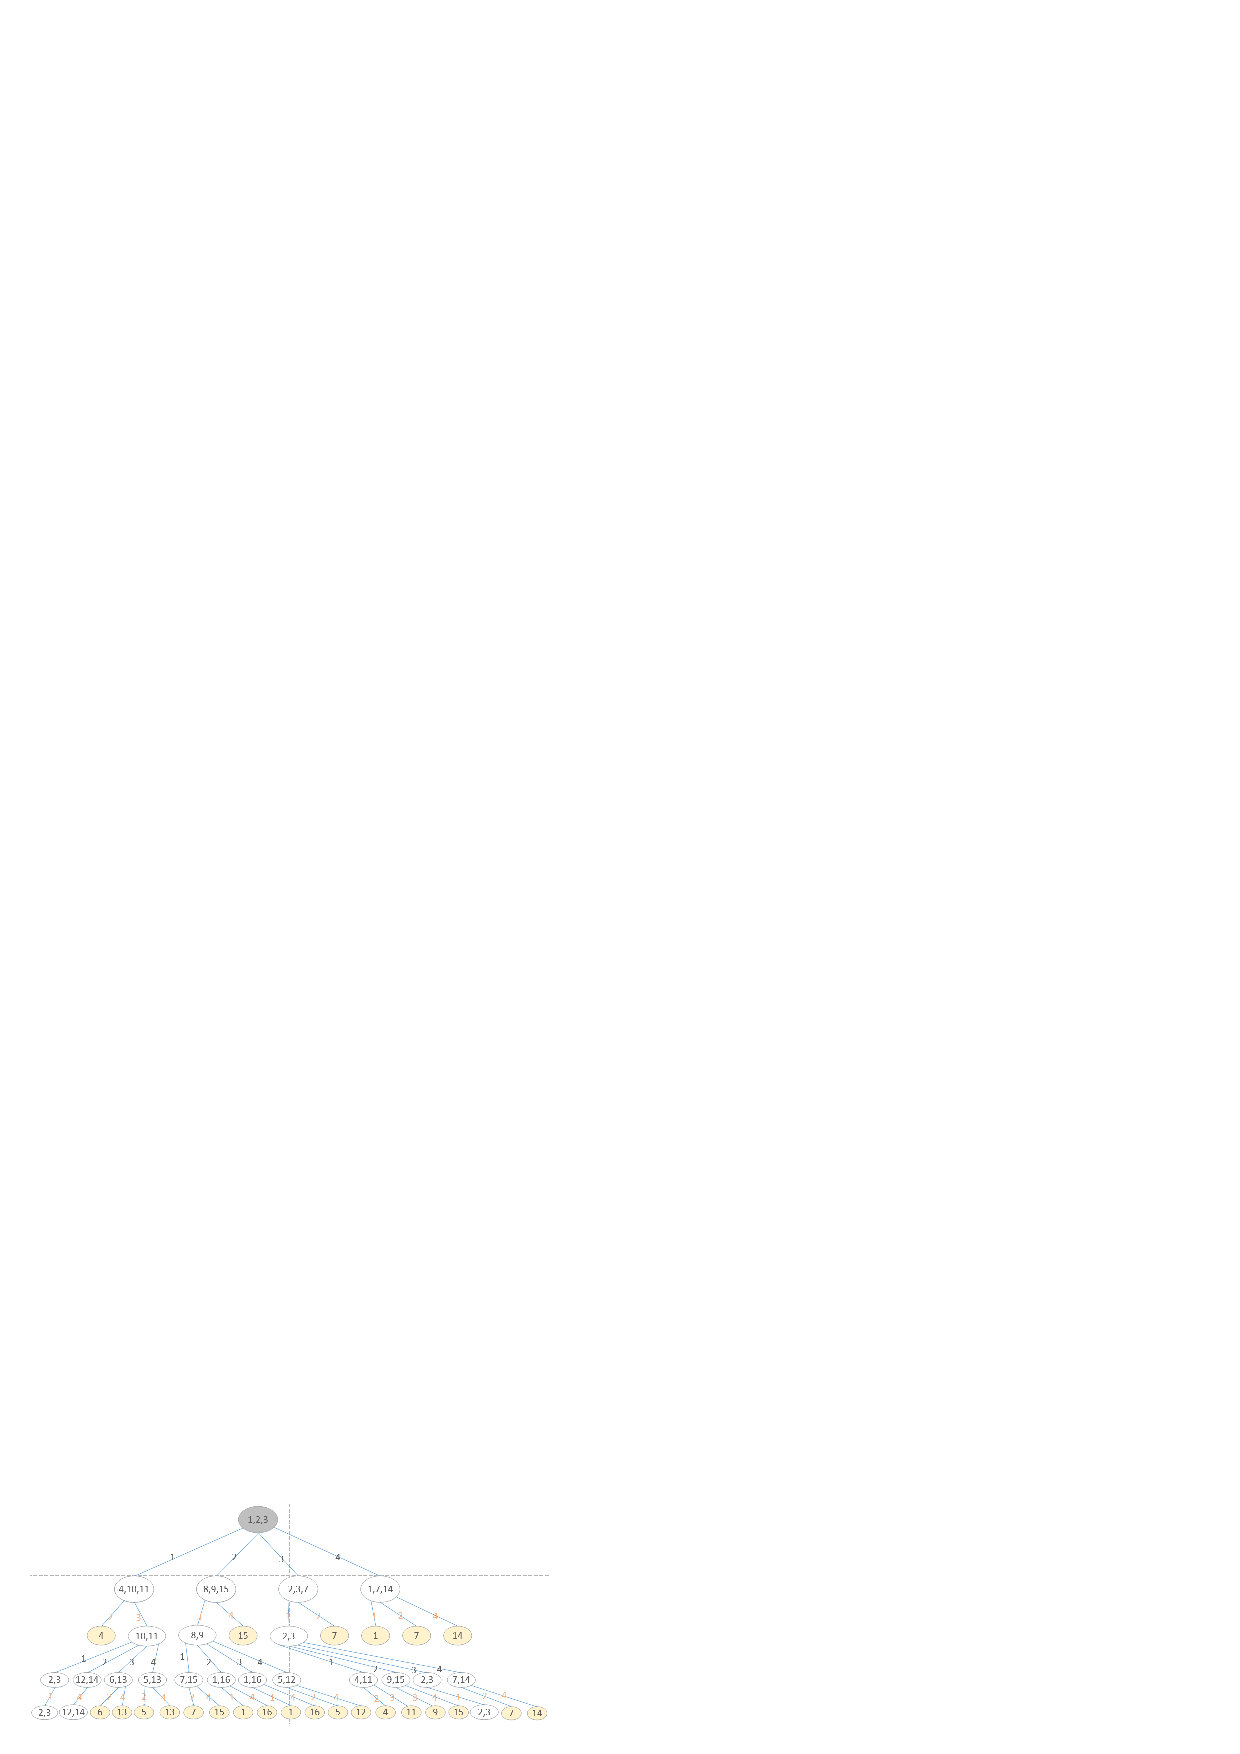
\includegraphics[scale=0.067]{figures/Fig3.png}}
	}}
      
      \caption{Branch of the super tree which represents $\{\delta_{16}^1,\delta_{16}^2,\delta_{16}^3\}$. The blue edges and orange edges show the observing output processes and deciding input processes, respectively. The yellow nodes are leaf nodes.}
      \label{fig:3}
   \end{figure}

In the {\em Definition \ref{def:super-tree}}. For a \BCN, we can only infer that the possible states set is $\Delta_N$ at the beginning, thus the root node of the super tree is $\Delta_N$. And then,  we can determine the state of the \BCN\ when the cardinal number of the possible states set turns into $1$. Therefore, the leaf nodes of the supertree are the nodes with cadinal number $1$. In the process of determining the initial state of a \BCN, we observe the output of the \BCN\ to derive the set of possible states at first. After that, we derive and decide the input and then derive the new possible states set of the \BCN. We alternately observe the output and then derive and decide the input untill we can determine the state of {\em BCN}. Therefore we use $\Ded\left(\mathsf{S}^i,\varepsilon, \mathsf{o}^j\right)$ to find child nodes for every $\mathsf{S}^i$ in $2k+1$ layer, and using $\Ded\left(\mathsf{S}^i,\mathsf{i}^p,\varepsilon\right)$ to find child nodes for every $\mathsf{S}^i$ in $2k+2$ layer. The formula 
\[|\Ded\left(\mathsf{S}^i,\varepsilon, \mathsf{o}^j\right)|>0\]
 ensures the node $\Ded\left(\mathsf{S}^i,\varepsilon, \mathsf{o}^j\right)$ is not empty. The formula 
 \[|\Ded\left(\mathsf{S}^i,\mathsf{i}^p,\varepsilon\right)|=|\mathsf{S}^i|\] 
 guarantee we can determine the state of \BCN\ in the end ({\em Section \ref{sec:online}} {\em Equation \ref{equ:12}}). Therefore, the paths to determine the initial state of a \BCN\ are described in the supertree, and then we can use it to determine the online observability for a \BCN.

Based on the definition of the supertree, we propose the supertree-based algorithm ({\em Algorithm.\ref{alg:3}}) to determine the online observability for \BCNs. 
%If we want to find all of the ways to determine the initial state of a \BCN, we have to build all leaf nodes for the super tree of this \BCN. This process takes many additional time and space overhead. Especially when there are loops in the tree such as the $\{\delta_{16}^2,\delta_{16}^3\}$ in fourth layer and the $\{\delta_{16}^2,\delta_{16}^3\}$ in fifth layer which will form a loop. In this case we can never build the complete tree, thus we need to check the existence of loops and omit them. There are also some nodes take the same set of state, that they will take some additional overhead as well. For instance there are two nodes take the same states set $\{\delta_{16}^1,\delta_{16}^{16}\}$ in the fifth layer. However, using super tree would be a lot easier than using directed graph if we only need to find a way to determine the initial state. For instance, when we find the leaf nodes $\delta_{16}^1$, $\delta_{16}^7$ and  $\delta_{16}^{14}$ in third layer by breadth-first algorithm, we can make sure that the states set $\{\delta_{16}^1,\delta_{16}^2,\delta_{16}^3\}$ is 1 step deterministic. Therefore, we could use this conclusion to determine the initial state of this \BCN. 
\begin{algorithm}[h]
\caption{Supertree-based algorithm}
\begin{algorithmic}[1]
\REQUIRE 
The algebraic form of \BCN
\ENSURE  
The super tree of \BCN
%\STATE  $k=1$ \
\STATE  $Ob=$ false %(The online observability of \BCN)\
%\STATE  $N_i$ (Node)\
%\STATE  $i_p$ (Input)\
\STATE  $NodesArray$ =$\Delta_N$\
%\STATE  $Sis$ (The suitable inputs set of $N_i$)\
%\STATE {\sf buildnode}(k)
%\STATE $k= k+1$
\WHILE {$Ob==$ false}
\STATE Build child nodes for $NodesArray$ by $\Ded\left(\mathsf{S}^i,\varepsilon, \mathsf{o}^j\right)$
\STATE $NodesArray=$ Child nodes of $NodeArray$ except leaf nodes
\STATE Check this \BCN\ by the super tree
\IF{\BCN\ is online observable}
\STATE $Ob=$ true
\ELSE
\STATE Build child nodes for $NodesArray$ by $\Ded\left(\mathsf{S}^i,\mathsf{i}^p,\varepsilon\right)$
\STATE $NodesArray=$ Child nodes of $NodeArray$
\ENDIF
\ENDWHILE
\STATE Delete uncertain branches
\STATE  $NodesArray$ =$\Delta_N$\
%\STATE return $Ob$
\STATE return $NodesArray$
\end{algorithmic}
 \label{alg:3}
\end{algorithm}

In the supertree-based algorithm we build trees by breadth first. We check the online observability of the \BCN\ by the supertree after $2k+2$ layer of the supertree was built for every $k\in  \mathbb{N}$. If the \BCN\ is online observable, then we stop building the supertree and delete the uncertain branches. Finally, we return the $NodesArray$ which is the root node of the supertree, and then we can determine the initial state of the \BCN\ by the supertree.

In order to better illustrate how to use the super tree to determine the online observability, we give the following example.
  
\begin{example}
In the \BCN\ mentioned in {\em Example \ref{exa:2}}. From the definition of online observability we need to determine whether the $\Ded\left(\Delta_N,\varepsilon,\mathsf{o}^j\right)$ is $K$-step deterministic for every  $\mathsf{o}^j\in \Delta_Q$ such that $|\Ded\left(\Delta_N,\varepsilon, \mathsf{o}^j\right)|> 0$. Therefore, we build child nodes for $\Delta_N$ by the $\Ded\left(\mathsf{S}^i,\varepsilon, \mathsf{o}^j\right)$. For instance, \[\Ded\left(\Delta_N,\varepsilon,\delta_{4}^1\right)=\{\delta_{16}^1,\delta_{16}^2,\delta_{16}^3\}\] and we can not determine whether $\{\delta_{16}^1,\delta_{16}^2,\delta_{16}^3\}$ is $K$-step deterministic or not at the beginning, and then we can not determine the online observability of this \BCN\ by the supertree now. Therefore we build child nodes for it, and then build child nodes for its child nodes as shown in the Fig.\ref{fig:3}. Then we check the second and third layer of this branch, we have the nodes $\{\delta_{16}^1\}$, $\{\delta_{16}^7\}$ and $\{\delta_{16}^{14}\}$ are $0$-step deterministic, and then we have the node $\{\delta_{16}^1,\delta_{16}^2,\delta_{16}^3\}$ is $1$-step deterministic. We use the same method to check other nodes, and then determine the online observability for the \BCN. Finally, we delete uncertain branches except the branches which can help us to determine online observability, such as the first branch ($\{\delta_{16}^{4},\delta_{16}^{10},\delta_{16}^{11}\}$). And then, the supertree can help us to determine the initial state of the \BCN.%We can also determine the initial state of this \BCN\ by this branch.The nodes represent the sets of possible states, the blue edges represent the processes of observing output, and the orange edges represent the processes of deriving and deciding input. Only the yellow nodes are the leaf nodes, thus this branch is not completed. %When we check the second and third layer of this branch, we have the nodes $\{\delta_{16}^1\}$, $\{\delta_{16}^7\}$ and $\{\delta_{16}^{14}\}$ are $K$-step deterministic, and then we have the node $\{\delta_{16}^1,\delta_{16}^2,\delta_{16}^3\}$ is $K$-step deterministic. We can also determine the initial state of this \BCN\ by this branch.

\end{example}   

However, if we want use the supertree-based algorithm to find all paths to determine the initial state of a \BCN. In this case, we need to check the nodes that appear multiple times in the supertree, and this nodes would take many additional time and space overhead. For instance, in the Fig.\ref{fig:3} there are two nodes take $\{\delta_{16}^1,\delta_{16}^{16}\}$ in the fourth layer. Moreover, the same nodes in a path will form a loop, the loops in the supertree will prevent us from building a complete tree. For example, there are the $\{\delta_{16}^2,\delta_{16}^3\}$ in fourth layer and the $\{\delta_{16}^2,\delta_{16}^3\}$ in fifth layer, and they would form a loop. With the shortcomings of the supertree, we propose the algorithm based on directed graph to help us find all paths to determine the initial state of a \BCN.
\subsection{Algorithm based on directed graph}
In order to improve the shortcomings of the supertree-based algorithm, we proposed the algorithm based on directed graph. The biggest difference of these two algorithms is the way how the  supertree and derected graph constructed. That supertree is built from the root node ($\Delta_N$) to leaf nodes (contain 1 state), while the derected graph is built from smallest nodes (contain 1 state) to largest node (contain largest number of states). In addition, there is not any repeated node in the derected graph because every node appears only once in the directed graph. What is more, even there are some loops in the derected graph, the loops would not prevent us from building the directed graph completely.

Therefore, we have the definition of directed graph for \BCNs.
\begin{definition}[Directed Graph]
Firstly, every node $\mathsf{S}^i$ in the directed graph is $K$-step deterministic, and there are no duplicate nodes in the graph. 

Secondly, for every node $\mathsf{S}^i$  and $|\mathsf{S}^i|>1$, we have that for every distinct two $\mathsf{s}^a, \mathsf{s}^b \in \mathsf{S}^i$, $H\mathsf{s}^a=H\mathsf{s}^b$. 

Finally, fot the edges of the directed graph. 
\begin{itemize}
 \item If $|\mathsf{S}^i|=1$, then there are not edge from it to other nodes.
 \item  If $|\mathsf{S}^i|>1$, and there are exist one edge $i_p$ from it to one nodes, then there exist $z\ge 1$ such that there are $z$ edges contain $i_p$ from it to nodes $\mathsf{S}^1,\ldots,\mathsf{S}^z$ that \[|\mathsf{S}^i|= |\mathsf{S}^1|+,\ldots,|\mathsf{S}^z|\] and \[\Ded\left(\mathsf{S}^i,i_p,\varepsilon\right)=\mathsf{S}^1\vee,\ldots,\vee \mathsf{S}^z.\]
 \end{itemize}

\end{definition}

From the {\em Lemma \ref{lemm:5}} in the {\em Section \ref{sec:online}}, we have that if the set of states $S_i$ is not $K$-step deterministic and $S_i\subset S_j$, then $S_j$ is not $K$-step deterministic. Therefore, we check whether the nodes with fewer states are $K$-step deterministic at first, and then we check whether the nodes with more states are $K$-step deterministic in the process of building the directed graph for a \BCN. Once we can find a node $S_i$ is not $K$-step deterministic, then we make sure that there exists $o_j \in \Delta_Q$ such that $|\Ded\left(\Delta_N,\varepsilon, o_j\right)|> 0$ and $S_i\subset \Ded\left(\Delta_N,\varepsilon, o_j\right)$, then $\Ded\left(\Delta_N,\varepsilon,o_j\right)$ is not $K$-step deterministic, and then this \BCN\ is not online observable. %Moreover, we can use the nodes with fewer states that are $k$-step deterministic to help us check the nodes with more states. For instance, if the node $S$ has two edges from it to two nodes $S_1$ and $S_2$, and we have $S_1$ and $S_2$ are $k$-step deterministic. In this case, we can make sure that the node $S$ is $k$-step deterministic.

With the definition of directed graph and the way to construct the derected graph. We propose the algorithm based on directed graph prsented in the {\em Algorithm.\ref{alg:1}}. And the {\em Algorithm.\ref{alg:2}} present the algorithm to build nodes which is used in the {\em Algorithm.\ref{alg:1}}.

\begin{algorithm}[h]
\caption{Algorithm based on directed graph}
\begin{algorithmic}[1]
\REQUIRE 
The algebraic forms of \BCN
\ENSURE  
The directed graph of \BCN
\STATE  $k=1$ %(The number of states in the nodes)\
\STATE  $Ob=$ true %(The online observability of \BCN)\
%\STATE  $N_i$ %(Node)\
%\STATE  $i_p$ %(Input)\
%\STATE  $NodesArray$% (Nodes array)\
%\STATE  $Sis$ %(The suitable inputs set of $N_i$)\
\STATE {\sf buildnode}(k)
\STATE $k= k+1$
\STATE $NodesArray=${\sf buildnode}(k)
\WHILE {$NodesArray!=$Null}

\FOR{each $S_i\in NodesArray$}
\IF{$k==2$}
\STATE $Sis$ = $\Delta_M$ 
\ELSE

\STATE Find $Sis$ by other nodes

\ENDIF
\FOR{each $i_p \in Sis$}
\STATE Check $S_i$ by $i_p$
\STATE Build edges for $S_i$ 
\ENDFOR
\IF {$S_i$ has not any edge.}
\STATE  $Ob=$ false 
\STATE return Null
\ENDIF
\ENDFOR
\STATE $k= k+1$
\STATE $NodesArray=${\sf buildnode}(k)
\ENDWHILE
%\STATE $Ob=1$ 
\STATE $NodesArray=${\sf buildnode}(k-1)
\STATE return $NodesArray$
\end{algorithmic}
 \label{alg:1}
\end{algorithm}
 %The algorithm to build nodes used in the Algorithm.\ref{alg:1} is shown in the Algorithm.\ref{alg:2}.
\begin{algorithm}[h!]
\caption{{\sf buildnode}(int k)}
\begin{algorithmic}[1]
\REQUIRE 
The number of states $k$
\ENSURE  
The nodes with $k$ states which with the same corresponding outputs %, and the outputs of $p$ states inside one node are the same.
%\STATE {\sf buildnode}(int p)
%\STATE  \{ 
%\dfSTATE $p=p+1$\
\STATE  Build all nodes with $p$ states %(whose outputs are the same)\

\IF{Failed to build} 
\STATE  return Null
\ELSE 
\STATE  Classify these nodes
\STATE Sort the states in these nodes
\STATE Sort these nodes%(For example, the nodes $\{\delta_{16}^1,\delta_{16}^2\}$, $\{\delta_{16}^1,\delta_{16}^3\}$ and $\{\delta_{16}^2,\delta_{16}^3\}$ shown in {\em Fig.\ref{fig:4}}. )
\STATE return nodes
\ENDIF 
%\STATE \}
\end{algorithmic}
 \label{alg:2}
\end{algorithm}
%%\newpage

There are some details in {\em Algorithm.\ref{alg:1}} and {\em Algorithm.\ref{alg:2}} are as follows:
\begin{itemize}
\item Build all nodes with $k$ states: Firstly, we classify all states by their corresponding outputs ($\Ded\left(\Delta_N,\varepsilon,o_j\right)$), then we have all of the states sets. The states set contains all states that with the same corresponding outputs. Secondly, we compare $k$ with the cardinal number $|\Ded\left(\Delta_N,\varepsilon,o_j\right)|$ of each states set we built before. If $k$ greater than $|\Ded\left(\Delta_N,\varepsilon,o_j\right)|$, then we could not get $k$ states from this states set. Else we can get $C_{|\Ded\left(\Delta_N,\varepsilon,o_j\right)|}^k$ sets with $k$ states from this states set. Finally, we use all of the sets of states found in second step to build nodes we need. 
 \item Sort the states in these nodes and sort these nodes: For example, the nodes $\{\delta_{16}^1,\delta_{16}^2\}$, $\{\delta_{16}^1,\delta_{16}^3\}$ and $\{\delta_{16}^2,\delta_{16}^3\}$ shown in Fig.\ref{fig:4}. We sort the states inside the nodes at first, and then sort the nodes by the states of them.
  \item Find $Sis$ by other nodes: From the {\em Lemma \ref{lemm:4}} and {\em Lemma \ref{lemm:3}} in the {\em Section \ref{sec:online}}, we have if $S_i\subset S_j$ then for any input $i$ wich can not make $S_i$ $K$-step deterministic, it can not make $S_j$ $K$-step deterministic either. Therefor, for the node $S_i$ with $k$ sorted states inside it, we can use the node with the first $k-1$ states of $S_i$ and the node with the last $k-1$ states of $S_i$ to find the suitable inputs set $Sis$ for $S_i$. For example, we can search correct inputs sets which make $\{\delta_{16}^4,\delta_{16}^5,\delta_{16}^6\}$ and $\{\delta_{16}^5,\delta_{16}^6,\delta_{16}^7\}$ $K$-step deterministic at first. After that, take the intersection of these sets to be the suitable inputs set of $\{\delta_{16}^4,\delta_{16}^5,\delta_{16}^6,\delta_{16}^7\}$. 
  \item Check $S_i$ by $i_p$: According to the order determined in previous steps, we check every node in order. If for one input $i_p\in Sis$ implies $|\Ded\left(S_i,i_p,\varepsilon\right)|<|S_i|$, we can make sure the $i_p$ is a wrong input. Else if for each $O_j \in \Delta_Q$, $|\Ded\left(S_i,i_p,o_j\right)|>0$ and $\Ded\left(S_i,i_p,o_j\right)$ is $K$-step deterministic then $I_j$ is a correct input. Therefore, we can connect the node $S_i$ to each node $\Ded\left(S_i,i_p,o_j\right)$ with directed edge. Else if there exist $o_j \in \Delta_Q$ and we can not make sure whether $\Ded\left(S_i,i_p,o_j\right)$ is $K$-step deterministic, then we check it in the next round. 
\end{itemize} 

\begin{figure}[thpb]
      \centering
      \framebox{\parbox{3in}{
		\centerline{\includegraphics[scale=0.090]{figures/Fig4.png}}
	}}
      
      \caption{Part of the directed graph which represents $\{\delta_{16}^1,\delta_{16}^2\}$, $\{\delta_{16}^1,\delta_{16}^3\}$ and $\{\delta_{16}^2,\delta_{16}^3\}$. The green, black, orange, blue edges show the inputs $\delta_4^1$, $\delta_4^2$, $\delta_4^3$ and $\delta_4^4$ respectively.}
      \label{fig:4}
   \end{figure}

What is more, based on the definitions of existing four types of observability, we can also use the directed graph to determine the existing second and fourth type of observability for \BCNs. 
\begin{itemize}
 \item Checking the existing second observability: When we try to build bottom layer and penultimate layer of the directed graph, and there are exist some nodes in penultimate layer has no edges from it to other nodes. 
 Therefore, there are distinct states $s_0$, ${s'}_0 \in \Delta_N$, and there does not exist any input sequence $I\in(\Delta_M)^p$ for any $p\in \mathbb{Z}_+$, such that $Hs_0=H{s'}_0$ implies $(HL)^p_{s_0}(I)\neq (HL)^p_{{s'}_0}(I)$.
 And then, this \BCN\ does not satisfy existing second observability.
 \item  Checking the existing fourth observability: When we try to build edges for every layer, and if there exist one node whose right inputs set is not $\Delta_M$, 
 then there exists an input sequence $I\in(\Delta_M)^{\infty}$ does not satisfy that for any distinct states $s_0$, ${s'}_0 \in \Delta_N$, $Hs_0=H{s'}_0$ implies $(HL)^{\infty}_{s_0}(I)\neq (HL)^{\infty}_{{s'}_0}(I)$. And then this \BCN\ does not satisfy existing fourth observability.
 \end{itemize}



\subsection{Complexity analysis}
As the algorithm by the directed graph is better than by supertree when we want to find all paths to determine the initial state of \BCNs. We analyze the complexity of this algorithm briefly in this paper. 
%We classify the states with their corresponding output . After that form the set of states set $\{\Ded\left(\Delta_N,\varepsilon,\delta_M^1\right), \Ded\left(\Delta_N,\varepsilon,\delta_M^2\right),\ldots,\Ded\left(\Delta_N,\varepsilon,\delta_M^M\right)\}$, then every element in a states set has the same corresponding output. For each \[S_i\in\{\Ded\left(\Delta_N,\varepsilon,\delta_M^1\right), \Ded\left(\Delta_N,\varepsilon,\delta_M^2\right),\ldots,\Ded\left(\Delta_N,\varepsilon,\delta_M^M\right)\}\] we have $Hs_k=\delta_{M}^i$ for every $s_k\in S_i$.
\begin{itemize}
\item Firstly, we need to calculate the number of layers in the directed graph i.e. the upper bound of the number ($k$) of the states of the nodes in the directed graph. We have that 
\begin{equation}
\begin{split}
k_{upb}= \max(|\Ded\left(\Delta_N,\varepsilon,\delta_M^1\right)|,\ldots,|\Ded\left(\Delta_N,\varepsilon,\delta_M^M\right)|).
\end{split}
\end{equation}
%The upper bound of the number of the states of the nodes in the directed graph $k_{upb}$ is the maximum value of $|\Ded\left(\Delta_N,\varepsilon,\delta_M^1\right)|,\ldots,|\Ded\left(\Delta_N,\varepsilon,\delta_M^M\right)|$, 
Because the states of the same nodes in the directed graph should have the same corresponding output. Therefore, the $k_{upb}$ indicates the number of layers in the directed graph, and it depends on the relationship between states and outputs of the \BCNs.

\item Secondly, we need to calculate the number of nodes which with $k$ states, we have that
\begin{equation}
\begin{split}
Non(k)= C_{|S_i|}^k+\ldots +C_{|S_p|}^k,
\end{split}
\end{equation}
where \[S_i\ldots,S_p\in\{\Ded\left(\Delta_N,\varepsilon,\delta_M^1\right),\ldots,\Ded\left(\Delta_N,\varepsilon,\delta_M^M\right)\}\] and $|S_i|,\ldots,|S_p|\ge k$. The $Non(k)$ indicates the number of nodes which built by the {\sf buildnode}(k) function, and it also depends on the relationship between states and outputs of the \BCNs.

\item Thirdly, we need to calculate the cardinal number of suitable inputs set of each node $|Sis(S_i)|$. If $|S_i|=2$ then $Sis(S_i)=\Delta_M$. If $|S_i|>2$ then $Sis(S_i)$ is derived by other nodes, therefore it depends on the updating rules of the \BCNs.

\item Finally, we need to calculate the time used to check whether a input which in the suitable inputs set of a node is a right input for this node $T(S_i, i_p)$, and it depends on the updating rules of the \BCNs\ as well.
 \end{itemize}

After completing the previous analysis, we calculate the complexity by layer by layer, then we have the time we need to determine the online observability.  
\begin{equation}
\begin{split}
T=\sum_{k=1}^{k_{upg}}\sum_{i=1}^{Non(k)}\sum_{p=1}^{Sis(S_i)}T(S_i, i_p)
\end{split}
\end{equation}
%\[T=\sum_{k=1}^{k_{upg}}\sum_{i=1}^{Non(k)}\sum_{p=1}^{Sis(S_i)}T(S_i, i_p)\]
%The cardinal number of suitable inputs set of a node depends on the cardinal number of this node and the other three nodes used to find the suitable inputs set for it. And the time used to check whether an input is a right input for a node also depends on the updating rules of {\em BCNs}.

%What is more, instead of taking $\Delta_M$ as the suitable inputs set for every node in thedirected graph, we use the other three nodes like $\{\delta_{16}^4,\delta_{16}^5,\delta_{16}^6\}$, $\{\delta_{16}^5,\delta_{16}^6,\delta_{16}^7\}$ and $\{\delta_{16}^4,\delta_{16}^7\}$ that are $k$-step deterministic to find the suitable inputs set for a node $\{\delta_{16}^4,\delta_{16}^5,\delta_{16}^6,\delta_{16}^7\}$ which with more than $2$ states. By this way we can  reduce the cardinal number of the suitable inputs set for every nodes with more than 2 states, and then reduce the time cost. 

%The reason why we can use this method is that only the input which make the subset of $\{\delta_{16}^4,\delta_{16}^5,\delta_{16}^6,\delta_{16}^7\}$ $k$-step deterministic will make the $\{\delta_{16}^4,\delta_{16}^5,\delta_{16}^6,\delta_{16}^7\}$ $k$-step deterministic. Furthermore, using these three nodes will be a good way to cover all the 2-state subsets (which with cardinal number $2$) of $\{\delta_{16}^4,\delta_{16}^5,\delta_{16}^6,\delta_{16}^7\}$. For every subset $s_i$ with cardinal number $2$ included in $\{\delta_{16}^4,\delta_{16}^5,\delta_{16}^6,\delta_{16}^7\}$ will included in $\{\delta_{16}^4,\delta_{16}^5,\delta_{16}^6\}$, $\{\delta_{16}^5,\delta_{16}^6,\delta_{16}^7\}$ or $\{\delta_{16}^4,\delta_{16}^7\}$. This conclusion can help us to select the nodes we need when we seek the suitable inputs set for a node. But it is hard to analyze the complexity of this method, and it makes the complexity analysis of the algorithm by directed graph harder.

From the definition, we know that the $k_{upb}$ and the $Non(k)$ are depend on the relationship between states and outputs of the \BCNs, and the $|Sis(S_i)|$ and $T(S_i, i_p)$ are depend on the updating rules of the \BCNs. Therefore, it is hard to give an accurate complexity of the algorithm by the number of the nodes of the \BCNs\ without the complete imformation of their updating rules. We just give a brief introduction of complexity analysis in this paper, and we would do more research about this problem in the furture.
%Because the states in a nodes will have the same corresponding output, so we have the upper bound of the number of the states in a directed graph nodes $k$: We classify the states with their corresponding output and form the set of states with the same corresponding output, the greatest cardinal number of these set would be the upper bound of $k$. 
\subsection{Determining initial state}

After introducing the algorithms to determine the online observability of the \BCNs, we present the way to determine the initial state of a \BCN\ by the directed graph. If a system described by \BCN\ is online observable, and the directed graph of it has been built, then we can determine the initial state of this system (or \BCN) in real time. In order to illustrate the process of determining the initial state of a \BCN, we give one example is as follows.
\begin{example}
In the \BCN\ mentioned in {\em Example \ref{exa:2}}. The process of determining its initial state is shown in the Fig.\ref{fig:5}. 
\begin{itemize}
  \item Firstly, we observe the output of the \BCN. If the output we observe is $\delta_4^1$ then we can derive that the set of possible initial states should be $\{\delta_{16}^1,\delta_{16}^2,\delta_{16}^3\}$, and we record them as the initial states and current states of the \BCN\ in the table. 
  \item Secondly, we derive and decide the input ($\delta_4^1$) and observe the output ($\delta_4^3$), then we can derive that the set possible current states ($\{\delta_{16}^{10},\delta_{16}^{11}\}$), and then we record them as current states set in their corresponding positions. 
 \item Repeat the second step untill the cardinal number of the possible states set turns into $1$. In that time we can determine the current state ($\delta_{16}^{6}$) and the corresponding initial state  ($\delta_{16}^{3}$) of the {\em BCN}.
\end{itemize} 
\end{example}   
%Input and output again and again 

\begin{figure}[thpb]
      \centering
      \framebox{\parbox{3in}{
		\centerline{\includegraphics[scale=0.266]{figures/Fig5.png}}
	}}
      
      \caption{The process of determing the initial state of BCNs, we change the values of current states by input and the output we observe. }
      \label{fig:5}
   \end{figure}
%\subsection{Less observation costs}

Although the way of determine the initial state of a \BCN\ by the directed graph is very brief, but it would help us present how to do some optimization in the process of determining the initial state of the \BCNs.


% !Mode\dots ``TeX:UTF-8''
% !TEX root = ../root.tex
\section{Optimization}
\label{sec:app}

In the {\em Section \ref{sec:online}}, we present that the online observability is the the necessary and sufficient condition of determine the initial state $\mathsf{s}(0)$ of the \BCNs. Therefore, it can help us determine the initial state of some \BCNs\ which can not be determined by the existing third and fourth observability. In addition, we can also use the online observability to some optimization, including finding the shortest path and avoid entering critical states in the process of determining the initial state of the \BCNs. %Because the output we observe is not sure, we use expected value and variance of the length of path and the times of entering critical states to help us to choose the input.If we research the systems described by \BCNs\ which are online observable but not satisfy the existing third and fourth observability, we can only use the online observability to determine their initial state in real time. If we have built the corresponding directed graphs for them, we can use the online observability to determine the initial state of these \BCNs. In addition, online observibility requires less observation costs for us to determine the initial state of some systems described by  \BCNs\ in real time. 


\subsection{Finding shortest path}
When we need to determine the initial state of a \BCN, an important aspect that we would consider is to find the shortest path to determine the initial state. In general, we can not find the shortest path definitely. Fortunately, we can use the directed graph to make the best decision. For the path to determine the initial state of the \BCNs, we introduce two functions $\Pe(\mathsf{S}(t),\mathsf{ i}^{i}(t))$ and $\Pv(\mathsf{S}(t),\mathsf{ i}^{i}(t))$ to describe its expected value and variance, respectively. The definition of them are as follows.

%We introduce two functions $Spe(S_i, I_i)$ and $Spv(S_i, I_i)$ to describe the expected value of the shortest path and variance of shortest path , $S_i$ is the possible states set and $I_i$ is the input we chose, the definition of $Spe(S_i, I_i)$ is as follows:\\
%With the $Spe(S_i, I_i)$ and $Spv(S_i, I_i)$ we can make the decision we like.


Some necessary statements before defining the functions $\Pe(\mathsf{S}(t),\mathsf{ i}^{i}(t))$ and $\Pv(\mathsf{S}(t),\mathsf{ i}^{i}(t))$:
\begin{itemize}
  \item $\mathsf{S}(t)$: the set of possible states.
  \item $\{\mathsf{ i}^{1}(t),\mathsf{ i}^{2}(t),\ldots, \mathsf{ i}^{z}(t)\}$ : the right inputs set of $\mathsf{S}(t)$;
  \item $\{\mathsf{S}^{1}(t+1),\mathsf{S}^{2}(t+1),\ldots, \mathsf{S}^{k}(t+1)\}$ : the set of state sets, and its elements corresponding to the possible outputs $\{\mathsf{o}^1(t+1),\mathsf{o}^2(t+1),\ldots,\mathsf{o}^k(t+1)\}$. As we choose the input $\mathsf{ i}^{i}(t)$ to determine the state $\mathsf{s}(t)$ of \BCN\ by $\mathsf{S}(t)$, where $\mathsf{ i}^{i}(t) \in \{\mathsf{ i}^{1}(t),\mathsf{ i}^{2}(t),\ldots, \mathsf{ i}^{z}(t)\}$.
 % \item the fourth one implies the third one, second one and first one.
\end{itemize} 
\begin{definition}[$\Spe(\mathsf{S}(t))$] \label{lspe}
 \[\Spe(\mathsf{S}(t))= \min(\Pe(\mathsf{S}(t), \mathsf{ i}^{1}(t)),\ldots,\Pe(\mathsf{S}(t), \mathsf{ i}^{z}(t))).\] 
\end{definition}

\begin{definition}[$\Pe(\mathsf{S}(t), \mathsf{ i}^{i}(t))$] \label{spe}

When the $|\mathsf{S}(t)|=1$,
\[\Pe(\mathsf{S}(t), \mathsf{ i}^{i}(t))=0\]  for every \[\mathsf{ i}^{i}(t) \in \{\mathsf{ i}^{1}(t),\mathsf{ i}^{2}(t),\ldots, \mathsf{ i}^{z}(t)\}.\] According to {\em Definition \ref{lspe}}, $\Spe(\mathsf{S}(t))=0$ if $|\mathsf{S}(t)|=1$. 

When the $|\mathsf{S}(t)|>1$, 
%and the $\{I_1,I_2,\cdots, I_p\}$ is the right inputs set of $S_i$. For every $I_i$ in $\{I_1,I_2,\cdots, I_p\}$ the $\{S_i^1,S_i^2,\cdots, S_i^k\}$ is a set of state sets whose elements corresponding to the possible outputs after input $I_i$, then 
we have that  
\[\Pe(\mathsf{S}(t), \mathsf{ i}^{i}(t))=1 +\frac{\sum_{j=1}^k \Spe(\mathsf{S}^{j}(t+1))|\mathsf{S}^{j}(t+1)|}{ |\mathsf{S}(t)|}\] 
%and 
%\[{\tt Spe}(S_i)= \min({\tt Pe}(S_i, I_1),{\tt Pe}(S_i, I_2),\cdots,{\tt Pe}(S_i, I_p))\]
\end{definition}

The function $\Spe(\mathsf{S}(t))$ to find the $\mathsf{ i}^{i}(t)$ from $\{\mathsf{ i}^{1}(t),\mathsf{ i}^{2}(t),\ldots, \mathsf{ i}^{z}(t)\}$ to calculat least $\Pe(\mathsf{S}(t), \mathsf{ i}^{i}(t))$ for $\mathsf{S}(t)$. From the definition of $\Pe(\mathsf{S}(t), \mathsf{ i}^{i}(t))$, we have that if $|\mathsf{S}(t)|=1$ then we can make sure the state of \BCNs. Thus we need not choose the input anymore to determine the state $\mathsf{s}(t)$ of \BCNs. Therefore, for any input the path expected value $\Pe(\mathsf{S}(t), \mathsf{ i}^{i}(t))$ would be $0$ and the shortest path expected value $\Spe(\mathsf{S}(t))$ also would be $0$. But if $|\mathsf{S}(t)|>1$ we still need to choose input and observe the output. Only by this way we can determine the state of of \BCNs. Thus we recursively define the $\Pe(\mathsf{S}(t), \mathsf{ i}^{i}(t))$ and $\Spe(\mathsf{S}(t))$ for each input $\mathsf{ i}^{i}(t)$ in the right inputs set. 

If we want to find the shortest path to determine the initial state of a \BCN, we can choose an input $\mathsf{ i}^{i}(t)$ with least $\Pe(\mathsf{S}(t), \mathsf{ i}^{i}(t))$ by the function $\Spe(\mathsf{S}(t))$. This input $\mathsf{ i}^{i}(t)$ may help us find the shortes path to determine the state. But the output of \BCNs\ we observe is uncertain after we choose the input $i_p$, hence selecting the $\mathsf{ i}^{i}(t)$ which with least $\Pe(\mathsf{S}(t), \mathsf{ i}^{i}(t))$ may leads to a very long path to determine the initial state of \BCNs. For better performce, we define the $\Pv(\mathsf{S}(t), \mathsf{ i}^{i}(t))$ to avoid risks.% The $\Pv(S, i_p)$ is defined in the similar way. %Hence we omit the details of the definition of $\Pv(S, i_p)$ in this paper. \\
\begin{definition}[$\Pv(\mathsf{S}(t), \mathsf{ i}^{i}(t))$] 
When the $|\mathsf{S}(t)|=1$, we have that
\[\Pv(\mathsf{S}(t), \mathsf{ i}^{i}(t))=0\]  for every \[\mathsf{ i}^{i}(t) \in \{\mathsf{ i}^{1}(t),\mathsf{ i}^{2}(t),\ldots, \mathsf{ i}^{z}(t)\}.\]  When the $|\mathsf{S}(t)|>1$, 
%and the $\{I_1,I_2,\cdots, I_p\}$ is the right inputs set of $S_i$. For every $I_i$ in $\{I_1,I_2,\cdots, I_p\}$ the $\{S_i^1,S_i^2,\cdots, S_i^k\}$ is a set of state sets whose elements corresponding to the possible outputs after input $I_i$, then 
we have that\\ $\Pv(\mathsf{S}(t), \mathsf{ i}^{i}(t))=$
\[\frac{\sum_{j=1}^k (\Spe(\mathsf{S}^{j}(t+1))-\Pe(\mathsf{S}(t), \mathsf{ i}^{i}(t))+1)^2 |\mathsf{S}^{j}(t+1)|}{ |\mathsf{S}(t)|}\]
%and 
%\[{\tt Spe}(S_i)= \min({\tt Pe}(S_i, I_1),{\tt Pe}(S_i, I_2),\cdots,{\tt Pe}(S_i, I_p))\]
\end{definition}

From the definition of the $\Pv(\mathsf{S}(t), \mathsf{ i}^{i}(t))$, we have that if the $\Pv(\mathsf{S}(t), \mathsf{ i}^{i}(t))$ of input $\mathsf{ i}^{i}(t)$ is not very large, the risk of choosing $\mathsf{ i}^{i}(t)$ would be not great either.
\subsection{Avoiding entering critical states}
In biological systems wich depiected by the \BCNs, some of the genes' states may corresponding to unfavorable or even dangerous situations \cite{Li2014Controllability}. So another important aspect that we consider is to avoid entering critical states in the process of determining the \BCN's initial state. Therefore, we also construct two functions $\Ce(\mathsf{S}(t), \mathsf{ i}^{i}(t))$ and $\Cv(\mathsf{S}(t), \mathsf{ i}^{i}(t))$ to describe expected value and variance of the times of entering critical states in the process determine the intial state of the \BCNs. The definition of $\Ce(\mathsf{S}(t), \mathsf{ i}^{i}(t))$ is as follows.\\
\begin{definition}[$\Lce(S)$] \label{lce}
\[\Lce(\mathsf{S}(t))= \min(\Ce(\mathsf{S}(t), \mathsf{ i}^{1}(t)),\ldots,\Ce(\mathsf{S}(t), \mathsf{ i}^{z}(t))).\]
\end{definition}
\begin{definition}[$\Ce(\mathsf{S}(t), \mathsf{ i}^{i}(t))$] 
When the $|S|=1$, we have \[\Ce(\mathsf{S}(t), \mathsf{ i}^{i}(t))=|\mathsf{S}(t) \cap \mathsf{S}_{cri} |,\]  for every \[\mathsf{ i}^{i}(t) \in \{\mathsf{ i}^{1}(t),\mathsf{ i}^{2}(t),\ldots, \mathsf{ i}^{z}(t)\}.\]  
According {\em Definition \ref{lce}}, %{\tt Spe}$(S_i)=0$ if $|S_i|=1$ 
\[\Lce(\mathsf{S}(t))=\Ce(\mathsf{S}(t), \mathsf{ i}^{i}(t))=|\mathsf{S}(t) \cap \mathsf{S}_{cri} |\] 
But when the $|S|>1$ 
%and the $\{I_1,I_2,\cdots, I_p\}$ is the right inputs set of $S_i$. For every $ I_i$ in $\{I_1,I_2,\cdots, I_p\}$ the $\{S_i^1,S_i^2,\cdots, S_i^k\}$ is a set of state sets whose elements corresponding to the possible outputs after input $I_i$, then 
we have that 
\[\Ce(\mathsf{S}(t), \mathsf{ i}^{i}(t))=|\mathsf{S}(t) \cap \mathsf{S}_{cri}| +\frac{\sum_{j=1}^k \Lce(\mathsf{S}^{j}(t+1))|\mathsf{S}^{j}(t+1)|}{ |\mathsf{S}(t)|} \] 
%and 
%\[{\tt Lce}(S_i)= \min({\tt Ce}(S_i, I_1),{\tt Ce}(S_i, I_2),\cdots,){\tt Ce}(S_i, I_p)\]
\end{definition}

Where $\mathsf{S}_{cri}$ is the critical states set of the \BCN\ we research. The definition of $\Ce(\mathsf{S}(t), \mathsf{ i}^{i}(t))$ has some difference with $\Pe(\mathsf{S}(t), \mathsf{ i}^{i}(t))$, because of the critical states set $\mathsf{S}_{cri}$. So that we can analyze the possibility of entering the critical states after we derived the possible states set of \BCNs, and we can get the definitions of $\Cv(\mathsf{S}(t), \mathsf{ i}^{i}(t))$ in the similar way. %We omit the details of the definition of $\Cv(S, i_p)$ in this paper as well. 

\begin{definition}[$\Cv(\mathsf{S}(t), \mathsf{ i}^{i}(t))$] 
When the $|S|=1$, we have that
$\Cv(\mathsf{S}(t), \mathsf{ i}^{i}(t))=0$ for every  \[\mathsf{ i}^{i}(t) \in \{\mathsf{ i}^{1}(t),\mathsf{ i}^{2}(t),\ldots, \mathsf{ i}^{z}(t)\}.\]   When the $|\mathsf{S}(t)|>1$, 
%and the $\{I_1,I_2,\cdots, I_p\}$ is the right inputs set of $S_i$. For every $I_i$ in $\{I_1,I_2,\cdots, I_p\}$ the $\{S_i^1,S_i^2,\cdots, S_i^k\}$ is a set of state sets whose elements corresponding to the possible outputs after input $I_i$, then 
we have that  \\
$\Cv(\mathsf{S}(t), \mathsf{ i}^{i}(t))=$
$$\frac{\sum_{j=1}^k (\Lce(\mathsf{S}^{j}(t+1))-\Ce(\mathsf{S}(t), \mathsf{ i}^{i}(t))+|\mathsf{S}(t) \cap \mathsf{S}_{cri}|)^2 |\mathsf{S}^{j}(t+1)|}{ |\mathsf{S}(t)|}$$
%and 
%\[{\tt Spe}(S_i)= \min({\tt Pe}(S_i, I_1),{\tt Pe}(S_i, I_2),\cdots,{\tt Pe}(S_i, I_p))\]
\end{definition}

The use of $\Ce(\mathsf{S}(t), \mathsf{ i}^{i}(t))$ and $\Cv(\mathsf{S}(t), \mathsf{ i}^{i}(t))$ are similar to $\Pe(\mathsf{S}(t), \mathsf{ i}^{i}(t))$ and $\Pv(\mathsf{S}(t), \mathsf{ i}^{i}(t))$ respectively. They help us avoid entering critical states of \BCNs\ in the process of determining the initial state of \BCNs. With these four functions $\Pe(\mathsf{S}(t), \mathsf{ i}^{i}(t))$, $\Pv(\mathsf{S}(t), \mathsf{ i}^{i}(t))$, $\Ce(\mathsf{S}(t), \mathsf{ i}^{i}(t))$ and $\Cv(\mathsf{S}(t), \mathsf{ i}^{i}(t))$, we can make the best decision we like. 

In the four existing types of observability, they have not property {\em interactivity}. This leads to we can not analyze the state of the \BCNs\ dynamically, hence it would be hard to do some optimation in the process of determining the initial state of the \BCNs. However, this problem can be solved by the online observability of the \BCNs\ better.
% !Mode\dots ``TeX:UTF-8''
% !TEX root = ../root.tex
\section{Conclusions}
\label{sec:con}
In this paper, firstly we proposed the online observability of {\em BCNs} and define its mathematical form. Secondly we use the super tree and directed graph to determine the online observability. After introduced the ways to determine the online observability we present some applications of the online observability of {\em BCNs} and talk about some advantages of it. %use it to try to find the shortest path and avoid entering critical states when we determining the initial state of {\em BCNs}. 

But even we use the directed graph, it is still hard to determine the  the online observability of a \BCN\ with a large number of nodes. Therefore, in the future we will try to separate the {\em BCNs}, and then determine their online observability respectively. Furthermore, we also want to try to use some knowledge about formal methods to earn scalability for {\em BCNs}. In addition to the theoretical aspect, the realistic application is also very important. Hence we will also try to find some realistic example which can be modeled by {\em BCNs}. So that we can research these realistic examples well and determine the online observability their models for better performance.
%%%%%%%%%%%%%%%%%%%%%%%%%%%%%%%%%%%%%%%%%%%%%%%%%%%%%%%%%%%%%%%%%%%%%%%%%%%%%%%%


%%%%%%%%%%%%%%%%%%%%%%%%%%%%%%%%%%%%%%%%%%%%%%%%%%%%%%%%%%%%%%%%%%%%%%%%%%%%%%%%

%References are important to the reader; therefore, each citation must be complete and correct. If at all possible, references should be commonly available publications.

 \bibliographystyle{IEEEtran} 

 \bibliography{bcn}
 


\end{document}
